\section{Methods}
\label{sec:hsolid-methods}

\subsection{Candidate Structure Optimization}
% modified from supp1-geo.tex
We consider three candidates C2/c-24, Cmca-4, Cmca-12 for the molecular phase and one candidate I4$_1$/amd for the atomic phase at $T=0K$ over the pressure range 350 GPa to 700 GPa. The static-lattice structures in the molecular phase are optimized using the vdW-DF functional at constant pressure.
As shown in Table~\ref{tab:hsolid-mol-press-rs}, all three molecular structures optimize to similar density at each pressure.
\begin{table}[h]
% 2020/05/18 notes, extracted from h11/analysis/11a_axes_pos.json
% 2020/06/03 updated using h117a/data/h117a_dft-geo.json
\centering
\begin{tabular}{cccccccccc}
\toprule
vdW-DF P(GPa) & 360 & 400 & 440 & 480 & 520 & 560 & 650 & 700 & 780 \\
\midrule
Cmca-4  & 1.303 & 1.283 & 1.265 & 1.250 & 1.235 & 1.222 & 1.196 & 1.183 & 1.164 \\
Cmca-12 & 1.306 & 1.286 & 1.268 & 1.252 & 1.237 & 1.224 & & & \\
C2/c-24 & 1.307 & 1.287 & 1.269 & 1.253 & 1.239 & 1.225 & 1.198 & 1.185 & \\
\bottomrule
\end{tabular}
\caption{vdW-DF pressure-density (expressed in $r_s$) relation of relaxed molecular candidate structures.}
\label{tab:hsolid-mol-press-rs}
\end{table}
In contrast, the atomic structure is optimized using DMC at constant volume.
While both constant-volume and constant-pressure optimizations are valid ways to find the minimum energy structure, the final density and pressure differ in general.
The DMC optimizations for the atomic structure have been carried out at evenly spaced $r_s$ values: $1.31$, $1.29$, $1.27$, $\dots$, $1.17$.
The density difference between the atomic and a molecular structure at a given pressure range is appreciably larger than the density difference among molecular-phase candidate structures.
Thus, when calculating energy and enthalpy differences, interpolation is needed further from data for the atomic structure than for the molecular structures.

All three molecular structures are monoclinic having $a=b\neq c$, $\alpha=\beta=90^\circ+\eta$, and $\gamma=120^\circ+\delta$. The slight distortions differ for each structure: $\eta=0$, $\delta\approx -0.5^\circ$ for Cmca-4, $\eta=0$, $\delta\approx+3.5^\circ$ for Cmca-12, and $\eta\approx0.1^\circ$, $\delta\approx-0.1^\circ$ for C2/c-24.
The evolution of the lattice parameters as a function of pressure are shown in Fig.~\ref{fig:hsolid-vdw-ca}(a).
Both $a$ and $c$ decrease with increasing pressure.
However, the $c/a$ ratio remains roughly constant at $1.062\pm0.003$ and $1.771\pm0.003$ for Cmca-12 and C2c-24, respectively.
In contrast, the $c/a$ ratio of the Cmca-4 structure decreases from $1.562$ at $350$ GPa to $1.530$ at $560$ GPa linearly with pressure.
Besides having a slightly different unit cell, the Cmca-4 structure has only one type of H$_2$ molecule, whereas Cmca-12 and C2/c each have two.
The bond length of the H$_2$ molecules in the optimized geometry is shown as a function of pressure in Fig.~\ref{fig:hsolid-vdw-ca}(b).

The vdW-DF optimized H$_2$ bond lengths of all three molecular structures are shown in Fig.~\ref{fig:hsolid-vdw-ca}(b).
The bond length in Cmca-4 is comparable to its isolated value of $1.4$ Bohr, whereas in C2/c-24 it is 3 to 4\% compressed.
One type of the H$_2$ molecules in Cmca-12 has pressure-sensitive bond length, increasing from $\sim 1.38$ Bohr at 360 GPa to $\sim 1.4$ Bohr at 560 GPa, while the other type has 3\% compressed bond length irrespective of pressure.

\begin{figure}[h]
\centering
\begin{minipage}{0.49\textwidth}
\centering
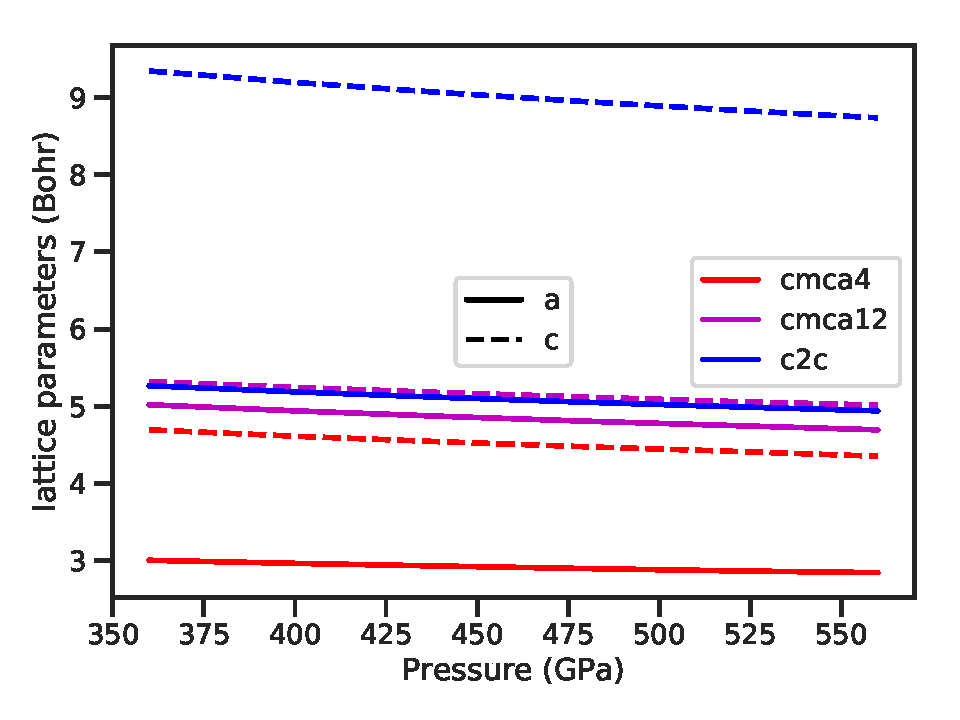
\includegraphics[width=\linewidth]{h11_mol-ca}
(a) $a$ and $c$ lattice parameters
\end{minipage}
\begin{minipage}{0.49\textwidth}
\centering
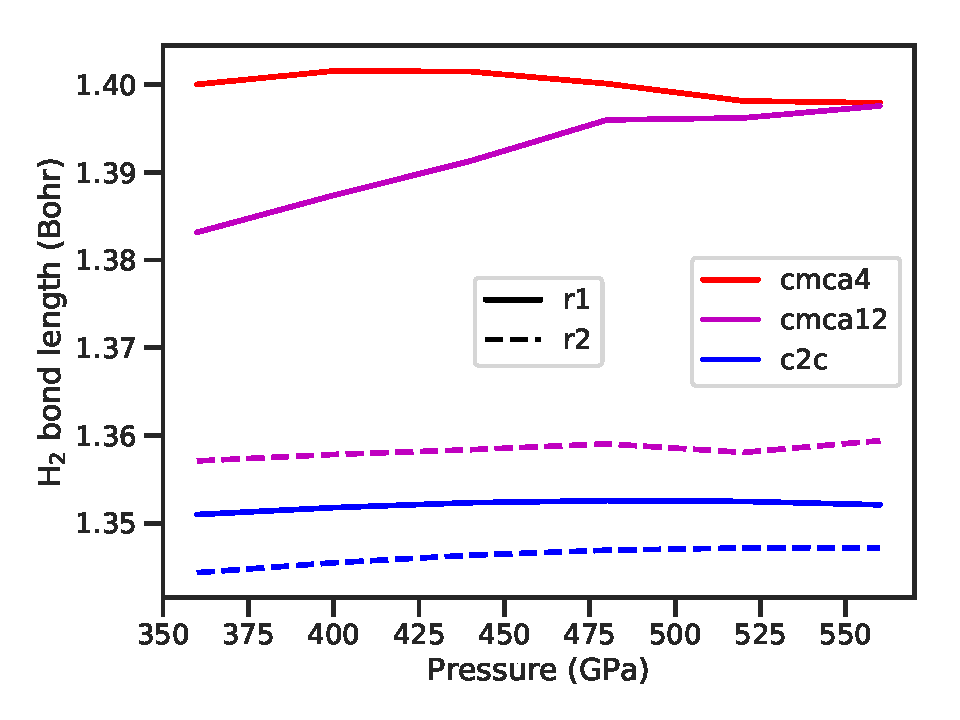
\includegraphics[width=\linewidth]{h11_mol-rb}
(b) H$_2$ bond length
\end{minipage}
\caption{vdW-DF optimized molecular candidate structures at target pressures. (a) lattice parameters (b) molecular bond length. C2/c and Cmca-12 each have two types of H$_2$ molecules, whereas Cmca-4 has only one.}
\label{fig:hsolid-vdw-ca}
\end{figure}

The atomic candidate structure I4$_1$/amd has only one free parameter, the $c/a$ ratio, at each density.
Therefore, we can afford to optimize its geometry using DMC within the clamped-ion approximation.
As shown in Fig.~\ref{fig:hsolid-i4-ca}, the DMC-optimized $c/a$ ratio is $4$ to $8$\% below the PBE-optimized ones.
It increases continuously as density increases, whereas the PBE-optimized $c/a$ ratio exhibits discontinuities around $r_s=1.21$ and $1.14$.
We fit $c/a$ as a linear function of $r_s$ to smooth out noise from the optimization process.

\begin{figure}[h]
\centering
\begin{minipage}{0.49\textwidth}
\centering
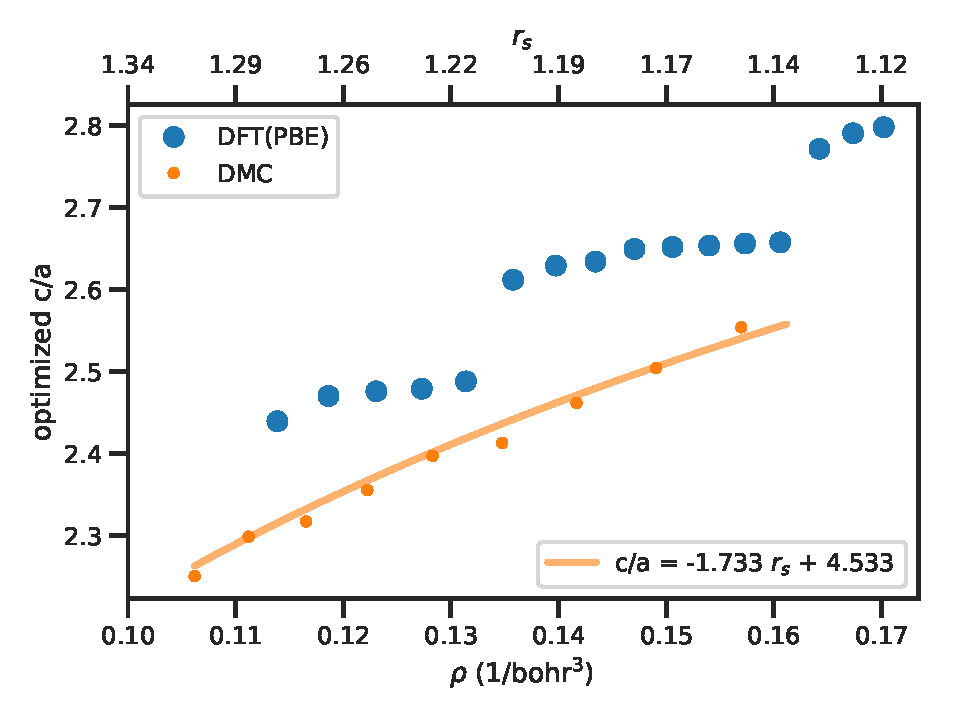
\includegraphics[width=\linewidth]{h117e_i4-ca}
\end{minipage}
\caption{DMC optimized atomic structure $c/a$ ratio as a function of density. The blue points are DFT(PBE) optimized $c/a$ ratios.}
\label{fig:hsolid-i4-ca}
\end{figure}

While the vdW-DF optimized structures in Ref.~\cite{McMinis2015} are not published, we can infer from the enthalpy-pressure relations that the same structures as in Ref.~\cite{McMinis2015} have been reproduced in this study. Figure~\ref{fig:dft-opt-geo} shows the enthalpy of each candidate structure relative to C2/c-24 at the vdW-DF static-lattice minimum. The results agree well with those from McMinis \textit{et al.}~\cite{McMinis2015} where available.
In comparison to predictions by Drummond \textit{et al.}~\cite{Drummond2015}, our C2/c structure is slightly more stable and Cmca-4 slightly less stable.
They used BLYP rather than vdW-DF functional, so differences are expected. In fact, it is encouraging to see two different functionals give similar results (within a few meV/p).

\begin{figure}[h]
\centering
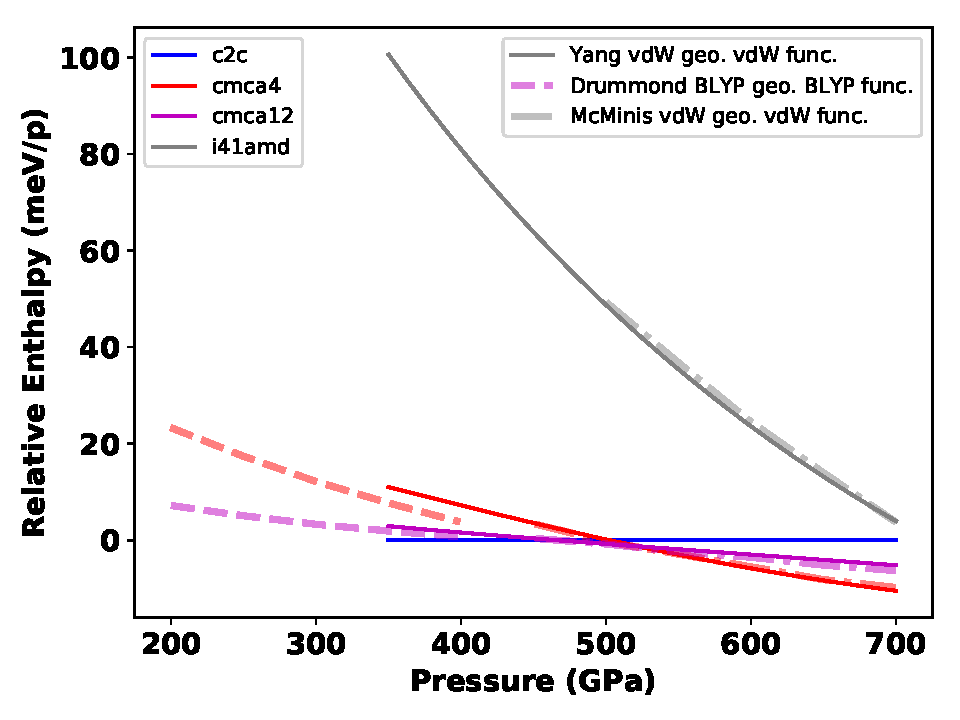
\includegraphics[width=0.6\columnwidth]{010a_dh-vs-p}
\caption{DFT(vdW-DF) static-lattice enthalpy of optimized structures relative to C2/c-24. Thin solid lines are enthalpies of the Cmca-4, Cmca-12 and I4$_1$/amd using our optimized structures. Dashed lines are DFT(BLYP) enthalpies of Cmca-4 and Cmca-12 from Drummond \textit{et al.}~\cite{Drummond2015}. Dash-dot lines are DFT(vdW-DF) enthalpies from McMinis \textit{et al.}~\cite{McMinis2015}.}
\label{fig:dft-opt-geo}
\end{figure}

\subsection{Supercell Construction}
% modified from supp2-static-qmc.tex
To reliably obtain QMC energies in the thermodynamic limit, we need to tile the optimized primitive cells to sufficiently large supercells so that pair correlation functions are converged.
The remaining finite-size error can be removed using methods discussed in Chap.~\ref{chap:fsc}.
The supercells also need to be small enough for dynamic-ion QMC to be practical.
In the end, we use 72-atom simulation cells for all QMC calculations.

Each simulation cell is tiled from the optimized unit cell using a non-diagonal \emph{supercell matrix}~\cite{Lloyd-Williams2015}, which is optimized to maximize the distance between minimum images.
A supercell matrix in 3D is a $3\times 3$ matrix of integers that map primitive lattice vectors $\bs{a}, \bs{b}, \bs{c}$ to supercell lattice vectors  $\bs{a}_s, \bs{b}_s, \bs{c}_s$
\begin{align}
\left(\begin{array}{c}
\bs{a}_s \\
\bs{b}_s \\
\bs{c}_s
\end{array}\right) =
\left(\begin{array}{ccc}
S_{11} & S_{12} & S_{13} \\
S_{21} & S_{22} & S_{23} \\
S_{31} & S_{32} & S_{33}
\end{array}\right)
\left(\begin{array}{c}
\bs{a} \\
\bs{b} \\
\bs{c}
\end{array}\right).
\end{align}
Once a supercell is chosen, the crystal structure can be created using the following cropping method: first, tile the atoms from the primitive cell a large number of times along each lattice vector, then crop out only the atoms that fall inside the supercell.
The total number of atoms in the supercell should be $\det(S)$ times that in the primitive cell.

\begin{figure}[h]
\centering
\begin{minipage}{0.49\textwidth}
\centering
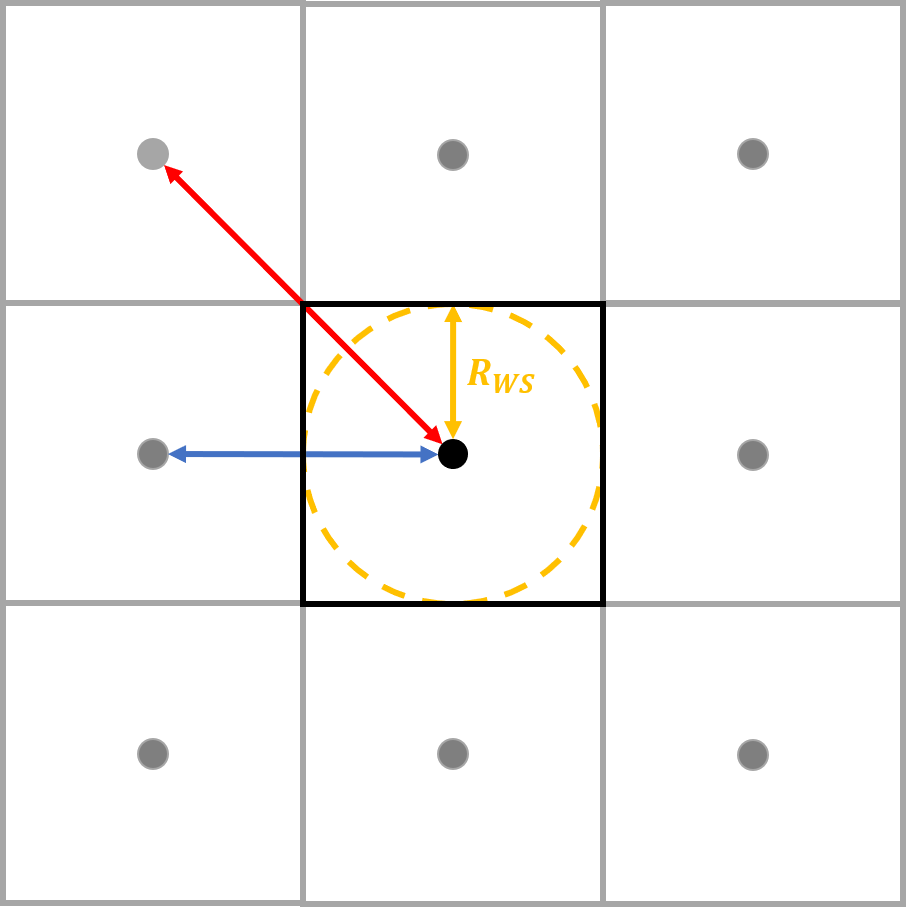
\includegraphics[width=0.6\linewidth]{supercell-square}\\
(a) square $a=2$ \AA
\end{minipage}
\begin{minipage}{0.49\textwidth}
\centering
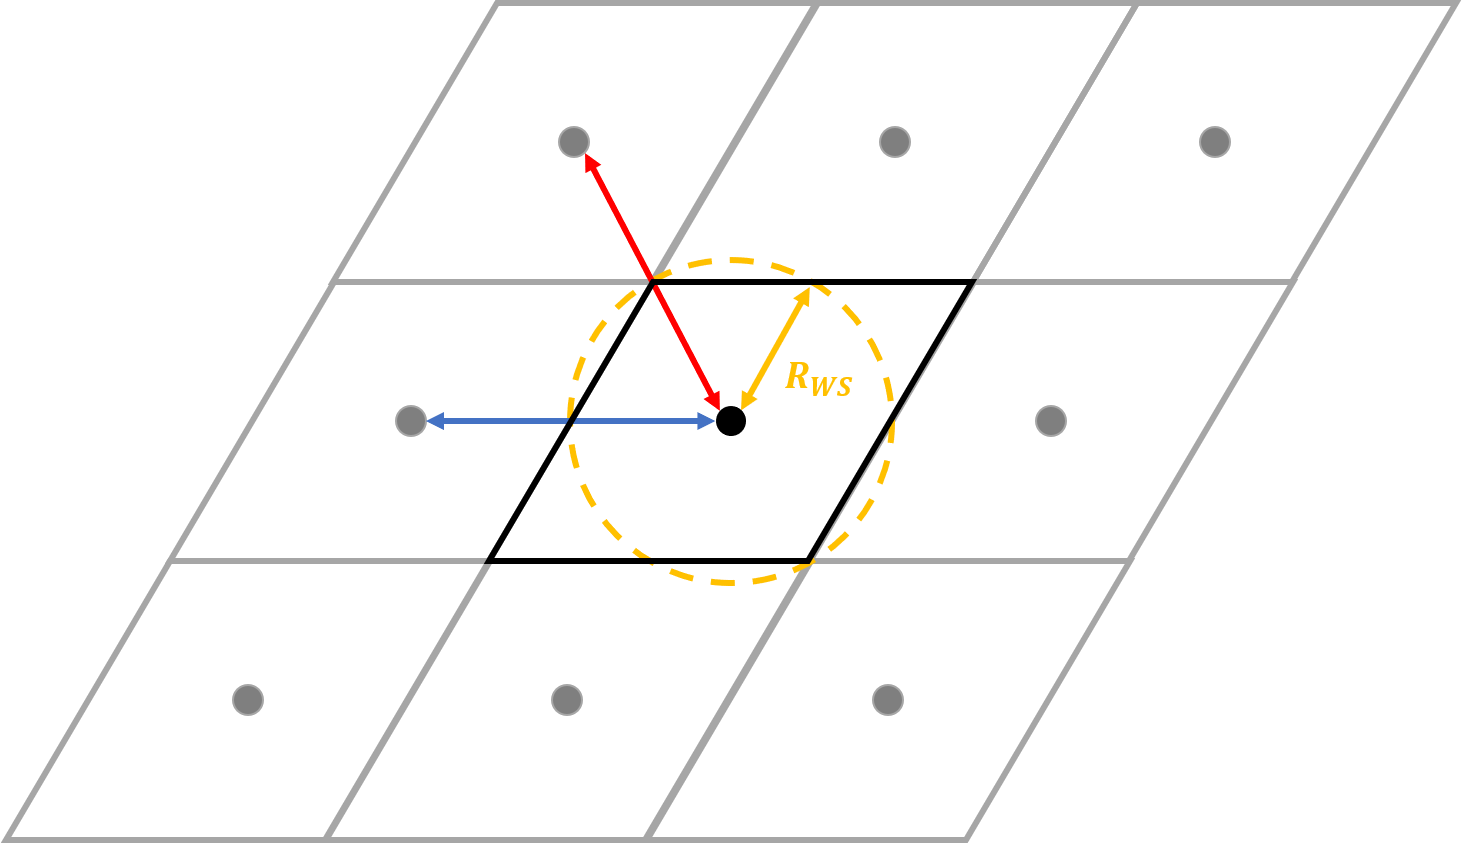
\includegraphics[width=\linewidth]{supercell-rhombus}\\
(b) rhombus $a=2.149$ \AA
\end{minipage}
\caption{Cubic vs. rhombus supercells. The black cell is the supercell. The gray cells are periodic images. The blue line points between nearest-neighbor images, while the red line between second-nearest neighbors. The yellow circle is the inscribed circle in the Wigner-Seitz cell (not shown) of the supercell.}
\label{fig:hsolid-square-vs-rhombus}
\end{figure}

Non-diagonal supercell matrices can be used to maximize the minimum image radius, radius of the real-space Wigner-Seitz cell $R_{WS}$.
As shown in Fig.~\ref{fig:hsolid-square-vs-rhombus}, a rhombus supercell provides a larger $R_{WS}$ than a square having the same area.
This is because the periodic images form a closed-packed lattice given a rhombus supercell.
If the primitive cell is square, then all diagonal supercell matrices result in square supercells. In contract, one can construct a rhombus-like supercell using a non-diagonal matrix.
A more useful application of non-diagonal supercell matrix is for accessing a particular momentum to address a certain excitation~\cite{Lloyd-Williams2015}, but that is beyond the scope of this study.

The chosen supercell matrices and their resulting image radii are shown in Table~\ref{tab:hsolid-tmat72} and Fig.~\ref{fig:cell-radius}, respectively.
The inscribing radius of each supercell $R_{sc}$ are also shown in Fig.~\ref{fig:cell-radius} to give a sense of how far each supercell is from being orthorhombic. An orthorhombic cell has $R_{WS} = R_{sc}$.
\begin{table}[h]
\centering
\caption{Optimized 72-atom non-diagonal supercell matrices.}
\label{tab:hsolid-tmat72}
\begin{tabular}{cccc}
\hline\hline
Cmca-4 & Cmca-12 & C2/c-24 & I4$_1$/amd \\
\hline
$\left(\begin{array}{rrr}
-1 &  2 &  1 \\
 2 & -1 &  1 \\
 3 &  3 &  0 \\
\end{array}\right)$ & $\left(\begin{array}{rrr}
 2 &  1 &  -1 \\
 2 &  1 &   1 \\
 -1 &  1 &  0 \\
\end{array}\right)$ & $\left(\begin{array}{rrr}
 2 &  1 &  0 \\
 1 &  2 &  0 \\
 0 &  0 &  1
\end{array}\right)$ & $\left(\begin{array}{rrr}
 2 & -2 &  1 \\
 2 &  3 &  0 \\
-2 &  1 &  1
\end{array}\right)$ \\
\hline\hline
\end{tabular}
\end{table}

\begin{figure}[h]
\centering
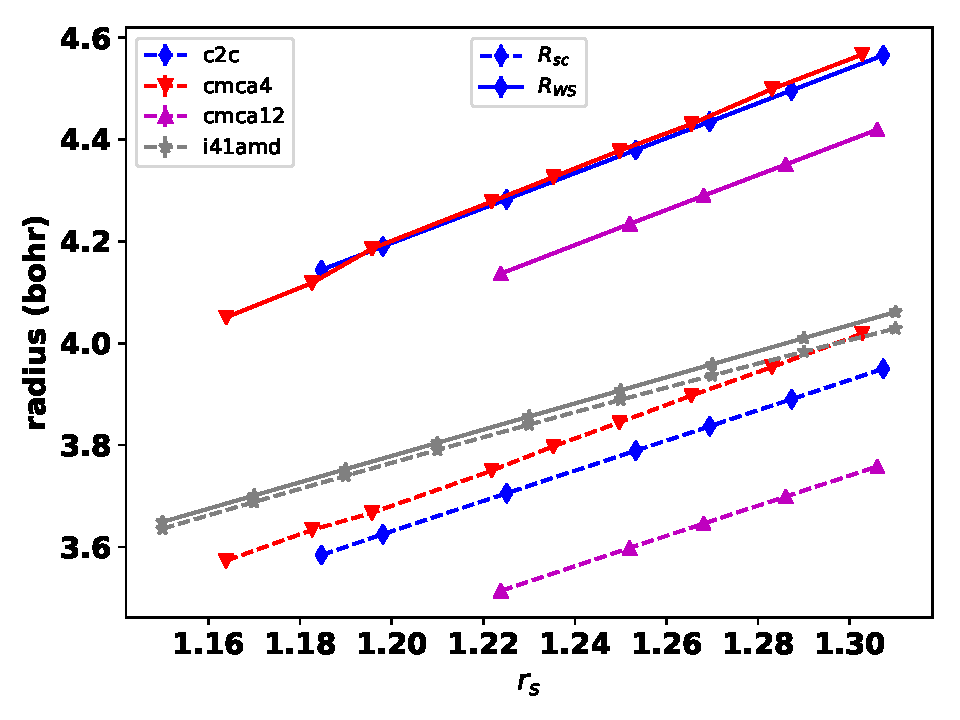
\includegraphics[width=0.6\columnwidth]{101a1_cell-radius}
\caption{Supercell radius as a function of density. $r_s$ is the Wigner-Seitz radius, which is determined by the average electron density $\frac{4\pi}{3}r_s=\rho$, where $\rho=N_e/\Omega$, with $\Omega$ the supercell volume. $R_{WS}$ is the radius of the real-space Wigner-Seitz cell of the supercell. $2R_{WS}$ is the minimum distance between periodic images. \label{fig:cell-radius}}
\end{figure}

%\section{Geometry Optimization}
% hsolid/11-refine-struct/a-ecut
The molecular structures are optimized in DFT using the vdW-DF functional. We use quantum ESPRESSO v5.3.0 to perform variable-cell geometry optimization at constant pressure. The atomic positions in the optimized unit cell are re-optimized at constant-volume. We use a Troullier-Martins pseudopotential with a core cutoff radius of $r_c=0.5$. The plane-wave cutoff energy is set to 160 Ry. Brillouin zone integration is performed using a shifted Monkhorst-Pack grid with $24^3$, $16^3$, $12^3$ points for the Cmca-4, Cmca-12, and C2/c-24 unit cells, respectively. %The effective number of atoms are 55296, 49152, and 41472, respectively.
Pressure is converged to 0.1 kbar (0.01 GPa). % Forces are converged to

The atomic structure is optimized in DMC. At each density, the $c/a$ parameter determines the I4$_1$/amd-4 ($c/a>1$) crystal structure. To optimize the $c/a$ parameter, we performed 5 DMC calculations at each density. These calculations form a grid in the lattice a-c parameter space as shown in Fig.~\ref{fig:i4-rs-ca}. Please see QMC section for details of the DMC calculations.
\begin{figure}[h]
% 2018-02-01_ani-press
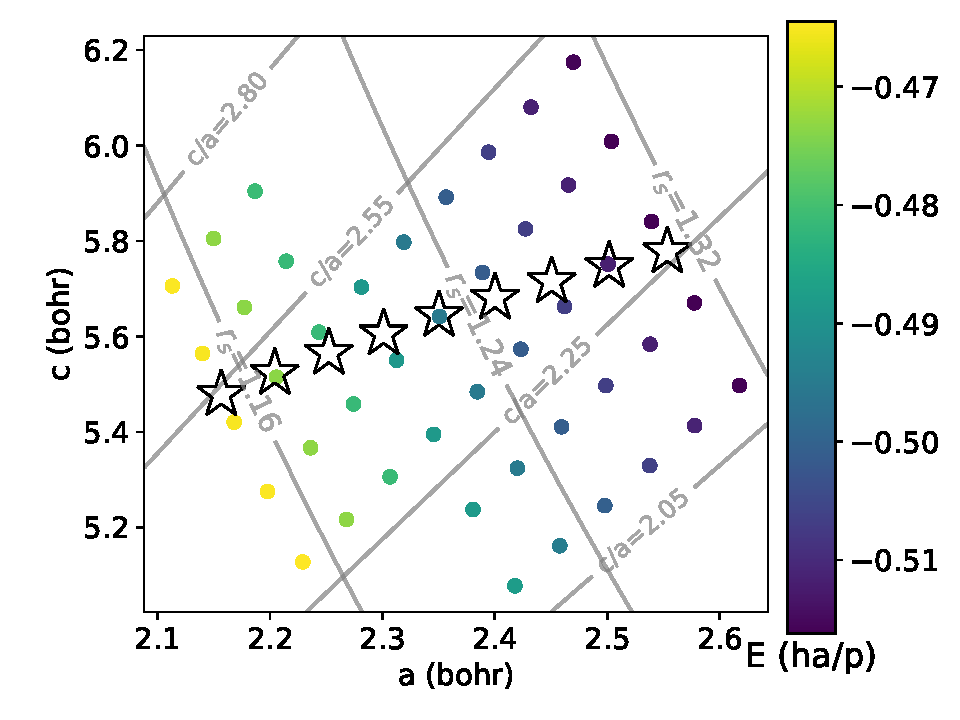
\includegraphics[width=0.8\columnwidth]{70_i4_ca_grid}
\caption{DMC calculations performed to optimize the atomic hydrogen solid structure. Each dot is a structure defined by the lattice parameters a and c. The color of each dot indicates the DMC energy. The gray contour lines mark structures with constant density or c/a ratio. Energy variation is dominated by density change. Energy variation in the c/a direction at fixed density is roughly quadratic around its minimum (black star). The black stars are the optimized geometries.\label{fig:i4-rs-ca}}.
\end{figure}

\section{Relative Enthalpy of Optimized Structures in DFT}
The enthalpies of the optimized crystal structures are calculated in DFT using the vdW-DF functional. As shown in Fig.~\ref{fig:dft-opt-geo},our relative enthalpies agree within 1.5 meV/p with those from McMinis et. al.. Our relative enthalpies for Cmca-12 agree within 1 mha/p with both those from Drummond et. al. and those from McMinis et. al.. Our relative enthalpy for Cmca-4 is higher than that of Drummond by 3.4 mha/p at 400 GPa. % Q/ Is the 3.4 mha/p difference due to structure or functional?
\begin{figure}[h]
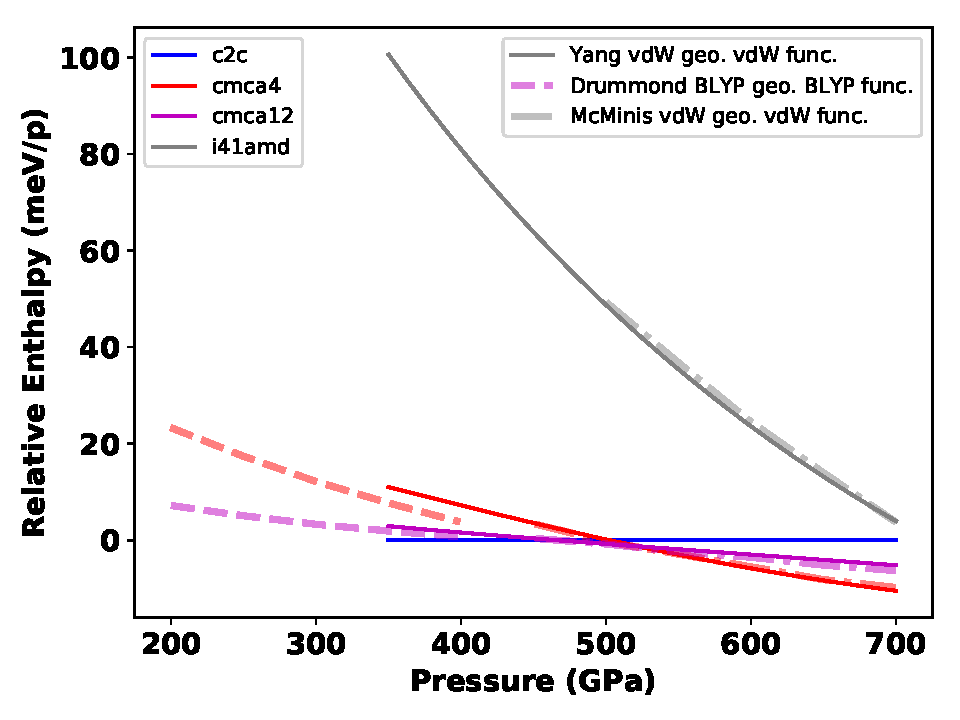
\includegraphics[width=0.8\columnwidth]{010a_dh-vs-p}
\caption{DFT(vdW-DF) enthalpy of optimized structures relative to C2/c-24. Thin solid lines are enthalpies of the Cmca-4, Cmca-12 and I4$_1$/amd using our optimized structures. Dashed lines are DFT(BLYP) enthalpies of Cmca-4 and Cmca-12 from Drummond et. al.. Dash-dot lines are DFT(vdW) enthalpies from McMinis et. al..\label{fig:dft-opt-geo}}
\end{figure}

%\subsection{Wavefunction}

All QMC calculations are performed using the QMCPACK code. We use Slater-Jastrow-Backflow (SJB) wavefunction. The orbitals in the Slater determinant are cusp-corrected DFT orbitals. The vdw-DF functional is used to generate orbitals for the molecular structures, whereas the PBE functional is used for the atomic structure. The orbital generating DFT runs have different settings compared to the geometry optimization runs.

To generate the orbitals, we perform DFT directly in the supercell. All calculations use the bare Coulomb interaction and a plane wave cutoff of 50 Ry. First, we run a self-consistent calculation to converge the charge density on a shifted $8^3$ Monkhorst-Pack grid. Second, we run a non-self-consistent calculation on an unshifted Monkhorst-Pack grid to generate the orbitals needed by all twists. $4^3$ twists are used for the molecular phase, while $6^3$ twists are used for the atomic phase. Finally, we divide each orbital by an electron-ion Jastrow wavefunction to remove the electron-ion cusp from the orbital. This electron-ion Jastrow wavefunction is constructed using Fourier components commensurate with the simulation cell (i.e. on the reciprocal lattice vectors of the simulation cell $\bs{G}_s$)
\begin{align}
J_{ei}(\bs{r}_j; \bs{R}) \propto& \exp\left\{ \text{iFFT}\left[ 
U_{\bs{k}}^{ep}  \left(\sum\limits_{J=1}^{N_p} \frac{e^{-i\bs{k}\cdot\bs{R}_J}}{N_p}  \right)
\right] \right\} \nonumber\\
\propto& \exp\left\{ 
\sum\limits_{\bs{k}\neq\bs{0}}^{\bs{k}\in\bs{G}_s} e^{i\bs{k}\cdot\bs{r}_j}~
U_{\bs{k}}^{ep} 
\left(\sum\limits_{J=1}^{N_p} \frac{e^{-i\bs{k}\cdot\bs{R}_J}}{N_p}  \right)
\right\},\label{eq:rpa-ep-jas}
\end{align}
where $\bs{r}_j$ is any single electron coordinate. $\bs{R}$ contains all ionic coordinates. $N_p$ is the number of protons. iFFT stands for ``inverse fast Fourier transform''. The Jastrow potential $U_{\bs{k}}^{ep}$ in eq.~(\ref{eq:rpa-ep-jas}) is chosen to be the RPA form written by Ceperley and Alder
\begin{align}
2U^{ep}_k = -a_k(1+a_k)^{-1/2},
\end{align}
where $a_k=\frac{12}{r_s^3k^4}$ in Hartree atomic units. $r_s$ is the Wigner-Seitz radius.

When a single-particle orbital is divided by eq.~(\ref{eq:rpa-ep-jas}), the electron-ion cusp is removed from the orbital. We re-introduce the electron-ion cusp in the Jastrow part of the trial wavefunction. 

There are 48 optimizable parameters in our wavefunction. We use short-range B-spline Jastrow pair potentials which are smoothly cut off at $R_{WS}$ (the image radius). There are three Jastrow potentials (uu, ud, ep) between up and up electrons, up and down electrons, electron and proton. We use short-range B-spline back flow transformation functions which are smoothly cut off $R_{WS}$. There are three backflow correlation functions (uu, ud, ep) similar to the Jastrow setup. Each B-spline has 8 optimizable knots.
\begin{comment}
\subsection{QMC Data}

At each density, we perform one VMC and two DMC calculations. Each QMC calculation is labeled by a series index. The VMC calculation is series 0. The first DMC calculation with a relatively large time step is series 1. The second DMC calculation with a relatively small time step is series 2. We post-process the raw results (series 0 - 2) to produce series 3 and 4. We linearly extrapolate the DMC results (series 1, 2) to zero time step and label the results series 3. We linearly extrapolate the VMC and the t=0 DMC results (series 0, 3) to obtain pure-estimator kinetic and potential energies and label them series 4.

Twist-average QMC energies are displayed in the following table. The dUlr column contains the many-body finite size correction which will be described in the next section.

\begin{table}[h]
\small
\begin{tabular}{llrrrllll}
\toprule
         &   &  timestep &  natom &      dUlr & LocalEnergy\_pp &    Variance\_pp &     Kinetic\_pp &    Potential\_pp \\
rs & series &           &        &           &                &                &                &                 \\
\midrule
1.163891 & 0 &    0.0300 &     72 &  0.005586 &    -0.47572(1) &     0.01380(2) &      0.9819(1) &      -1.4576(1) \\
         & 1 &    0.0030 &     72 &  0.005417 &   -0.477138(9) &    0.013719(9) &     0.98177(9) &     -1.45890(8) \\
         & 2 &    0.0015 &     72 &  0.005404 &    -0.47712(1) &     0.01374(1) &      0.9822(1) &    -1.45933(10) \\
         & 3 &    0.0000 &     72 &  0.005391 &    -0.47711(2) &     0.01374(1) &      0.9827(2) &      -1.4598(2) \\
         & 4 &    0.0000 &     72 &  0.005213 &    -0.47711(2) &     0.01374(1) &      0.9834(2) &      -1.4598(2) \\
1.182675 & 0 &    0.0300 &     72 &  0.005455 &    -0.48354(1) &     0.01347(2) &      0.9581(1) &      -1.4416(1) \\
         & 1 &    0.0030 &     72 &  0.005269 &   -0.484951(9) &    0.013408(8) &     0.95828(9) &     -1.44323(9) \\
         & 2 &    0.0015 &     72 &  0.005287 &    -0.48496(1) &     0.01342(1) &      0.9585(1) &      -1.4434(1) \\
         & 3 &    0.0000 &     72 &  0.005305 &    -0.48496(2) &     0.01342(1) &      0.9587(2) &      -1.4436(2) \\
         & 4 &    0.0000 &     72 &  0.005170 &    -0.48496(2) &     0.01342(1) &      0.9592(2) &      -1.4436(2) \\
1.195717 & 0 &    0.0300 &     72 &  0.005373 &   -0.488647(6) &    0.012795(9) &     0.94365(7) &     -1.43230(7) \\
         & 1 &    0.0030 &     72 &  0.005188 &   -0.490019(9) &    0.012688(8) &     0.94357(9) &     -1.43361(9) \\
         & 2 &    0.0015 &     72 &  0.005183 &   -0.490017(9) &    0.012707(9) &     0.94391(9) &     -1.43394(9) \\
         & 3 &    0.0000 &     72 &  0.005178 &    -0.49002(2) &    0.012707(9) &      0.9443(2) &      -1.4343(2) \\
         & 4 &    0.0000 &     72 &  0.004997 &    -0.49002(2) &    0.012707(9) &      0.9449(2) &      -1.4343(2) \\
1.221845 & 0 &    0.0300 &     72 &  0.005135 &   -0.497976(6) &    0.012288(9) &     0.91589(7) &     -1.41386(7) \\
         & 1 &    0.0030 &     72 &  0.004973 &   -0.499383(8) &    0.012232(9) &     0.91531(9) &     -1.41469(9) \\
         & 2 &    0.0015 &     72 &  0.004998 &   -0.499352(8) &    0.012255(9) &     0.91567(9) &     -1.41501(9) \\
         & 3 &    0.0000 &     72 &  0.005023 &    -0.49932(2) &    0.012255(9) &      0.9160(2) &      -1.4153(2) \\
         & 4 &    0.0000 &     72 &  0.004922 &    -0.49932(2) &    0.012255(9) &      0.9162(2) &      -1.4153(2) \\
1.235307 & 0 &    0.0300 &     72 &  0.005067 &   -0.502414(6) &     0.01188(1) &     0.90195(6) &     -1.40436(7) \\
         & 1 &    0.0030 &     72 &  0.004900 &   -0.503809(8) &    0.011814(8) &     0.90131(9) &     -1.40508(9) \\
         & 2 &    0.0015 &     72 &  0.004908 &   -0.503783(9) &    0.011793(9) &     0.90181(9) &     -1.40559(9) \\
         & 3 &    0.0000 &     72 &  0.004915 &    -0.50376(2) &    0.011793(9) &      0.9023(2) &      -1.4061(2) \\
         & 4 &    0.0000 &     72 &  0.004776 &    -0.50376(2) &    0.011793(9) &      0.9027(2) &      -1.4061(2) \\
1.249707 & 0 &    0.0300 &     72 &  0.004887 &   -0.506825(6) &     0.01274(2) &     0.88739(7) &     -1.39422(7) \\
         & 1 &    0.0030 &     72 &  0.004748 &   -0.508268(9) &    0.012682(9) &      0.8869(1) &     -1.39525(9) \\
         & 2 &    0.0015 &     72 &  0.004765 &   -0.508273(9) &    0.012696(9) &     0.88747(9) &     -1.39574(9) \\
         & 3 &    0.0000 &     72 &  0.004783 &    -0.50828(2) &    0.012696(9) &      0.8880(2) &      -1.3962(2) \\
         & 4 &    0.0000 &     72 &  0.004690 &    -0.50828(2) &    0.012696(9) &      0.8886(2) &      -1.3962(2) \\
1.265425 & 0 &    0.0300 &     72 &  0.004870 &   -0.511407(6) &     0.01158(1) &     0.87289(6) &     -1.38430(7) \\
         & 1 &    0.0030 &     72 &  0.004684 &   -0.512853(8) &    0.011519(8) &     0.87292(9) &     -1.38577(9) \\
         & 2 &    0.0015 &     72 &  0.004697 &   -0.512872(8) &    0.011541(8) &     0.87333(9) &     -1.38621(9) \\
         & 3 &    0.0000 &     72 &  0.004710 &    -0.51289(2) &    0.011541(8) &      0.8738(2) &      -1.3866(2) \\
         & 4 &    0.0000 &     72 &  0.004565 &    -0.51289(2) &    0.011541(8) &      0.8746(2) &      -1.3866(2) \\
1.283017 & 0 &    0.0300 &     72 &  0.004733 &   -0.516220(6) &    0.011305(9) &     0.85757(7) &     -1.37379(7) \\
         & 1 &    0.0030 &     72 &  0.004574 &   -0.517656(8) &    0.011240(9) &     0.85753(9) &     -1.37518(9) \\
         & 2 &    0.0015 &     72 &  0.004575 &   -0.517673(9) &    0.011251(8) &     0.85793(9) &     -1.37560(9) \\
         & 3 &    0.0000 &     72 &  0.004575 &    -0.51769(2) &    0.011251(8) &      0.8583(2) &      -1.3760(2) \\
         & 4 &    0.0000 &     72 &  0.004430 &    -0.51769(2) &    0.011251(8) &      0.8591(2) &      -1.3760(2) \\
1.302685 & 0 &    0.0300 &     72 &  0.004606 &   -0.521222(6) &    0.010863(8) &     0.84146(7) &     -1.36269(7) \\
         & 1 &    0.0030 &     72 &  0.004447 &   -0.522642(8) &    0.010795(7) &     0.84153(8) &     -1.36415(8) \\
         & 2 &    0.0015 &     72 &  0.004452 &   -0.522665(8) &    0.010810(8) &     0.84172(8) &     -1.36439(8) \\
         & 3 &    0.0000 &     72 &  0.004457 &    -0.52269(2) &    0.010810(8) &      0.8419(2) &      -1.3646(2) \\
         & 4 &    0.0000 &     72 &  0.004322 &    -0.52269(2) &    0.010810(8) &      0.8424(2) &      -1.3646(2) \\
\bottomrule
\end{tabular}

\caption{Cmca-4}
\end{table}

\begin{table}[h]
\small
\begin{tabular}{llrrrllll}
\toprule
         &   &  timestep &  natom &      dUlr & LocalEnergy\_pp &     Variance\_pp &     Kinetic\_pp &   Potential\_pp \\
rs & series &           &        &           &                &                 &                &                \\
\midrule
1.223839 & 0 &    0.0300 &     72 &  0.005398 &   -0.498582(6) &     0.013259(9) &     0.91712(7) &    -1.41570(7) \\
         & 1 &    0.0030 &     72 &  0.005121 &   -0.500194(9) &     0.013059(9) &     0.91759(9) &    -1.41781(9) \\
         & 2 &    0.0015 &     72 &  0.005123 &   -0.500189(9) &     0.013063(9) &     0.91791(9) &    -1.41810(9) \\
         & 3 &    0.0000 &     72 &  0.005125 &    -0.50018(2) &     0.013063(9) &      0.9182(2) &     -1.4184(2) \\
         & 4 &    0.0000 &     72 &  0.004868 &    -0.50018(2) &     0.013063(9) &      0.9193(2) &     -1.4184(2) \\
1.251971 & 0 &    0.0300 &     72 &  0.005113 &   -0.507671(7) &     0.013093(9) &     0.89092(7) &    -1.39859(7) \\
         & 1 &    0.0030 &     72 &  0.004888 &   -0.509262(8) &     0.012973(9) &     0.89079(8) &    -1.40004(8) \\
         & 2 &    0.0015 &     72 &  0.004888 &   -0.509253(8) &     0.012967(9) &     0.89147(9) &    -1.40072(9) \\
         & 3 &    0.0000 &     72 &  0.004888 &    -0.50924(2) &     0.012967(9) &      0.8922(2) &     -1.4014(2) \\
         & 4 &    0.0000 &     72 &  0.004676 &    -0.50924(2) &     0.012967(9) &      0.8934(2) &     -1.4014(2) \\
1.268116 & 0 &    0.0300 &     72 &  0.005012 &   -0.512485(6) &     0.011951(8) &     0.87796(7) &    -1.39044(7) \\
         & 1 &    0.0030 &     72 &  0.004777 &   -0.514038(9) &     0.011822(9) &     0.87737(8) &    -1.39142(8) \\
         & 2 &    0.0015 &     72 &  0.004761 &   -0.514071(9) &     0.011820(9) &     0.87791(9) &    -1.39197(9) \\
         & 3 &    0.0000 &     72 &  0.004745 &    -0.51410(2) &     0.011820(9) &      0.8785(2) &     -1.3925(2) \\
         & 4 &    0.0000 &     72 &  0.004490 &    -0.51410(2) &     0.011820(9) &      0.8789(2) &     -1.3925(2) \\
1.286021 & 0 &    0.0300 &     72 &  0.004894 &    -0.51743(1) &      0.01155(1) &      0.8626(1) &     -1.3800(1) \\
         & 1 &    0.0030 &     72 &  0.004676 &   -0.518992(8) &     0.011411(9) &     0.86249(9) &    -1.38150(9) \\
         & 2 &    0.0015 &     72 &  0.004645 &    -0.51902(1) &    0.011398(10) &      0.8624(1) &     -1.3814(1) \\
         & 3 &    0.0000 &     72 &  0.004614 &    -0.51905(2) &    0.011398(10) &      0.8623(2) &     -1.3813(2) \\
         & 4 &    0.0000 &     72 &  0.004351 &    -0.51905(2) &    0.011398(10) &      0.8620(2) &     -1.3813(2) \\
1.306029 & 0 &    0.0300 &     72 &  0.004704 &   -0.522568(6) &      0.01157(2) &     0.84694(7) &    -1.36950(7) \\
         & 1 &    0.0030 &     72 &  0.004498 &   -0.524120(9) &     0.011457(9) &     0.84641(8) &    -1.37052(8) \\
         & 2 &    0.0015 &     72 &  0.004515 &   -0.524133(8) &     0.011450(8) &     0.84684(9) &    -1.37098(9) \\
         & 3 &    0.0000 &     72 &  0.004531 &    -0.52415(2) &     0.011450(8) &      0.8473(2) &     -1.3714(2) \\
         & 4 &    0.0000 &     72 &  0.004370 &    -0.52415(2) &     0.011450(8) &      0.8476(2) &     -1.3714(2) \\
\bottomrule
\end{tabular}

\caption{Cmca-12}
\end{table}

\begin{table}[h]
\small
\begin{tabular}{llrrrllll}
\toprule
         &   &  timestep &  natom &      dUlr & LocalEnergy\_pp &     Variance\_pp &     Kinetic\_pp &   Potential\_pp \\
rs & series &           &        &           &                &                 &                &                \\
\midrule
1.184674 & 0 &    0.0300 &     72 &  0.005670 &    -0.48422(1) &      0.01254(2) &      0.9616(1) &     -1.4459(1) \\
         & 1 &    0.0030 &     72 &  0.005413 &   -0.485676(9) &    0.012399(10) &     0.96117(9) &    -1.44684(9) \\
         & 2 &    0.0015 &     72 &  0.005411 &    -0.48568(1) &    0.012389(10) &      0.9616(1) &     -1.4473(1) \\
         & 3 &    0.0000 &     72 &  0.005409 &    -0.48569(2) &    0.012389(10) &      0.9620(2) &     -1.4477(2) \\
         & 4 &    0.0000 &     72 &  0.005167 &    -0.48569(2) &    0.012389(10) &      0.9624(2) &     -1.4477(2) \\
1.198103 & 0 &    0.0300 &     72 &  0.005490 &    -0.48946(1) &      0.01307(2) &      0.9490(1) &     -1.4384(1) \\
         & 1 &    0.0030 &     72 &  0.005271 &   -0.490925(8) &     0.012934(9) &     0.94809(9) &    -1.43904(8) \\
         & 2 &    0.0015 &     72 &  0.005273 &    -0.49093(1) &      0.01295(1) &      0.9487(1) &     -1.4396(1) \\
         & 3 &    0.0000 &     72 &  0.005275 &    -0.49093(2) &      0.01295(1) &      0.9493(2) &     -1.4402(2) \\
         & 4 &    0.0000 &     72 &  0.005080 &    -0.49093(2) &      0.01295(1) &      0.9496(2) &     -1.4402(2) \\
1.225107 & 0 &    0.0300 &     72 &  0.005412 &   -0.499215(7) &     0.011982(8) &     0.92039(7) &    -1.41960(7) \\
         & 1 &    0.0030 &     72 &  0.005135 &   -0.500680(9) &     0.011825(8) &     0.91983(9) &    -1.42051(9) \\
         & 2 &    0.0015 &     72 &  0.005138 &   -0.500694(9) &     0.011830(8) &     0.92029(9) &    -1.42099(9) \\
         & 3 &    0.0000 &     72 &  0.005140 &    -0.50071(2) &     0.011830(8) &      0.9207(2) &     -1.4215(2) \\
         & 4 &    0.0000 &     72 &  0.004886 &    -0.50071(2) &     0.011830(8) &      0.9211(2) &     -1.4215(2) \\
1.253286 & 0 &    0.0300 &     72 &  0.005220 &   -0.508316(6) &      0.01170(1) &     0.89260(7) &    -1.40092(7) \\
         & 1 &    0.0030 &     72 &  0.004942 &   -0.509765(9) &      0.01152(1) &     0.89257(8) &    -1.40232(8) \\
         & 2 &    0.0015 &     72 &  0.004929 &   -0.509798(8) &     0.011498(8) &      0.8929(1) &    -1.40282(9) \\
         & 3 &    0.0000 &     72 &  0.004917 &    -0.50983(2) &     0.011498(8) &      0.8933(2) &     -1.4033(2) \\
         & 4 &    0.0000 &     72 &  0.004634 &    -0.50983(2) &     0.011498(8) &      0.8940(2) &     -1.4033(2) \\
1.269426 & 0 &    0.0300 &     72 &  0.005052 &   -0.513065(6) &     0.011097(9) &     0.87708(7) &    -1.39014(7) \\
         & 1 &    0.0030 &     72 &  0.004806 &   -0.514529(8) &     0.010948(8) &     0.87756(9) &    -1.39209(9) \\
         & 2 &    0.0015 &     72 &  0.004799 &   -0.514517(8) &     0.010939(8) &     0.87786(9) &    -1.39238(9) \\
         & 3 &    0.0000 &     72 &  0.004792 &    -0.51451(2) &     0.010939(8) &      0.8782(2) &     -1.3927(2) \\
         & 4 &    0.0000 &     72 &  0.004549 &    -0.51451(2) &     0.010939(8) &      0.8792(2) &     -1.3927(2) \\
1.287311 & 0 &    0.0300 &     72 &  0.004946 &   -0.518053(6) &     0.010534(8) &     0.86353(7) &    -1.38158(7) \\
         & 1 &    0.0030 &     72 &  0.004690 &   -0.519484(9) &     0.010371(8) &     0.86319(9) &    -1.38267(9) \\
         & 2 &    0.0015 &     72 &  0.004683 &   -0.519499(9) &     0.010369(7) &     0.86374(8) &    -1.38325(9) \\
         & 3 &    0.0000 &     72 &  0.004675 &    -0.51951(2) &     0.010369(7) &      0.8643(2) &     -1.3838(2) \\
         & 4 &    0.0000 &     72 &  0.004423 &    -0.51951(2) &     0.010369(7) &      0.8651(2) &     -1.3838(2) \\
1.307314 & 0 &    0.0300 &     72 &  0.004801 &    -0.52318(1) &      0.01054(2) &      0.8471(1) &     -1.3703(1) \\
         & 1 &    0.0030 &     72 &  0.004552 &   -0.524617(8) &     0.010398(8) &     0.84732(9) &    -1.37196(9) \\
         & 2 &    0.0015 &     72 &  0.004552 &    -0.52464(1) &      0.01039(1) &      0.8478(1) &     -1.3724(1) \\
         & 3 &    0.0000 &     72 &  0.004552 &    -0.52466(2) &      0.01039(1) &      0.8483(2) &     -1.3729(2) \\
         & 4 &    0.0000 &     72 &  0.004322 &    -0.52466(2) &      0.01039(1) &      0.8494(2) &     -1.3729(2) \\
\bottomrule
\end{tabular}

\caption{C2/c-24}
\end{table}

\begin{table}[h]
\small
\begin{tabular}{llrrrllll}
\toprule
     &   &  timestep &  natom &      dUlr &  LocalEnergy\_pp &     Variance\_pp &      Kinetic\_pp &   Potential\_pp \\
rs & series &           &        &           &                 &                 &                 &                \\
\midrule
1.15 & 0 &    0.0300 &     72 &  0.006282 &    -0.468339(9) &      0.02039(2) &      0.97451(7) &    -1.44285(7) \\
     & 1 &    0.0030 &     72 &  0.005793 &     -0.47074(1) &      0.01978(1) &      0.97496(9) &    -1.44572(9) \\
     & 2 &    0.0015 &     72 &  0.005797 &     -0.47073(1) &      0.01980(1) &      0.97534(9) &    -1.44607(9) \\
     & 3 &    0.0000 &     72 &  0.005800 &     -0.47072(3) &      0.01980(1) &       0.9757(2) &     -1.4464(2) \\
     & 4 &    0.0000 &     72 &  0.005371 &     -0.47072(3) &      0.01980(1) &       0.9769(2) &     -1.4464(2) \\
1.17 & 0 &    0.0300 &     72 &  0.006168 &    -0.476700(9) &      0.02044(2) &      0.94912(7) &    -1.42582(8) \\
     & 1 &    0.0030 &     72 &  0.005678 &    -0.479108(9) &      0.01981(1) &      0.94928(7) &    -1.42839(7) \\
     & 2 &    0.0015 &     72 &  0.005659 &    -0.479149(9) &      0.01981(1) &      0.94962(7) &    -1.42876(7) \\
     & 3 &    0.0000 &     72 &  0.005639 &     -0.47919(2) &      0.01981(1) &       0.9499(2) &     -1.4291(2) \\
     & 4 &    0.0000 &     72 &  0.005158 &     -0.47919(2) &      0.01981(1) &       0.9508(2) &     -1.4291(2) \\
1.19 & 0 &    0.0300 &     72 &  0.005965 &   -0.484386(10) &      0.02117(2) &      0.92299(7) &    -1.40738(7) \\
     & 1 &    0.0030 &     72 &  0.005520 &     -0.48679(1) &      0.02062(2) &      0.92317(9) &    -1.40994(9) \\
     & 2 &    0.0015 &     72 &  0.005508 &     -0.48683(1) &      0.02062(2) &      0.92352(9) &    -1.41035(9) \\
     & 3 &    0.0000 &     72 &  0.005497 &     -0.48687(3) &      0.02062(2) &       0.9239(2) &     -1.4108(2) \\
     & 4 &    0.0000 &     72 &  0.005077 &     -0.48687(3) &      0.02062(2) &       0.9248(2) &     -1.4108(2) \\
1.21 & 0 &    0.0300 &     72 &  0.005837 &     -0.49145(1) &       0.0197(2) &       0.9000(1) &     -1.3914(1) \\
     & 1 &    0.0030 &     72 &  0.005390 &   -0.493853(10) &      0.01908(1) &      0.89966(7) &    -1.39351(7) \\
     & 2 &    0.0015 &     72 &  0.005394 &   -0.493893(10) &      0.01908(1) &      0.89987(7) &    -1.39376(7) \\
     & 3 &    0.0000 &     72 &  0.005398 &     -0.49393(2) &      0.01908(1) &       0.9001(2) &     -1.3940(2) \\
     & 4 &    0.0000 &     72 &  0.005002 &     -0.49393(2) &      0.01908(1) &       0.9002(2) &     -1.3940(2) \\
1.23 & 0 &    0.0300 &     72 &  0.005709 &     -0.49788(1) &      0.01952(6) &       0.8772(1) &     -1.3751(1) \\
     & 1 &    0.0030 &     72 &  0.005260 &    -0.500351(9) &      0.01906(1) &      0.87668(7) &    -1.37703(7) \\
     & 2 &    0.0015 &     72 &  0.005243 &    -0.500363(9) &      0.01905(1) &      0.87711(7) &    -1.37748(7) \\
     & 3 &    0.0000 &     72 &  0.005226 &     -0.50038(2) &      0.01905(1) &       0.8775(2) &     -1.3779(2) \\
     & 4 &    0.0000 &     72 &  0.004781 &     -0.50038(2) &      0.01905(1) &       0.8779(2) &     -1.3779(2) \\
1.25 & 0 &    0.0300 &     72 &  0.005701 &     -0.50380(1) &      0.01725(2) &       0.8546(1) &     -1.3584(1) \\
     & 1 &    0.0030 &     72 &  0.005192 &    -0.506311(9) &    0.016644(10) &      0.85476(7) &    -1.36107(7) \\
     & 2 &    0.0015 &     72 &  0.005195 &    -0.506295(9) &    0.016635(10) &      0.85502(7) &    -1.36131(7) \\
     & 3 &    0.0000 &     72 &  0.005199 &     -0.50628(2) &    0.016635(10) &       0.8553(2) &     -1.3615(2) \\
     & 4 &    0.0000 &     72 &  0.004741 &     -0.50628(2) &    0.016635(10) &       0.8560(2) &     -1.3615(2) \\
1.27 & 0 &    0.0300 &     72 &  0.005504 &     -0.50918(1) &      0.01858(2) &       0.8365(1) &     -1.3457(1) \\
     & 1 &    0.0030 &     72 &  0.005037 &    -0.511700(9) &      0.01807(1) &      0.83566(7) &    -1.34736(7) \\
     & 2 &    0.0015 &     72 &  0.005031 &   -0.511705(10) &      0.01808(1) &      0.83584(7) &    -1.34755(7) \\
     & 3 &    0.0000 &     72 &  0.005025 &     -0.51171(2) &      0.01808(1) &       0.8360(2) &     -1.3477(2) \\
     & 4 &    0.0000 &     72 &  0.004588 &     -0.51171(2) &      0.01808(1) &       0.8355(2) &     -1.3477(2) \\
1.29 & 0 &    0.0300 &     72 &  0.005491 &     -0.51409(1) &      0.01634(2) &     0.81539(10) &     -1.3295(1) \\
     & 1 &    0.0030 &     72 &  0.004980 &   -0.516579(10) &      0.01577(1) &      0.81540(7) &    -1.33198(7) \\
     & 2 &    0.0015 &     72 &  0.004968 &    -0.516601(9) &      0.01579(1) &      0.81556(7) &    -1.33216(7) \\
     & 3 &    0.0000 &     72 &  0.004955 &     -0.51662(2) &      0.01579(1) &       0.8157(2) &     -1.3323(2) \\
     & 4 &    0.0000 &     72 &  0.004467 &     -0.51662(2) &      0.01579(1) &       0.8160(2) &     -1.3323(2) \\
1.31 & 0 &    0.0300 &     72 &  0.005418 &     -0.51851(1) &      0.01569(2) &       0.7983(1) &     -1.3168(1) \\
     & 1 &    0.0030 &     72 &  0.004889 &    -0.521027(9) &    0.015035(10) &      0.79760(7) &    -1.31862(7) \\
     & 2 &    0.0015 &     72 &  0.004880 &    -0.521046(9) &     0.015035(9) &      0.79801(7) &    -1.31906(7) \\
     & 3 &    0.0000 &     72 &  0.004871 &     -0.52106(2) &     0.015035(9) &       0.7984(2) &     -1.3195(2) \\
     & 4 &    0.0000 &     72 &  0.004371 &     -0.52106(2) &     0.015035(9) &       0.7985(2) &     -1.3195(2) \\
\bottomrule
\end{tabular}

\caption{I4$_1$/amd}
\end{table}

\subsection{Many-body Finite Size Correction}

We use the fluctuating structure factor $\delta S(\bs{k})\equiv \braket{(\rho_{\bs{k}}-\bar{\rho}_{\bs{k}})(\rho_{-\bs{k}}-\bar{\rho}_{-\bs{k}})}$ to calculate many-body finite size correction (FSC) to the potential energy. The integrand is cut off using optimized long-range Coulomb potential in reciprocal space $v_k^{lr}$
\begin{align}
\Delta V^{lr} = \left[\int - \sum\right] \frac{1}{2}v^{lr}_k \delta S(\bs{k}).
\end{align}
Total energy FSC ($\Delta E$) is a sum of kinetic ($\Delta T$) and potential ($\Delta V$) corrections regardless of whether mixed-estimator (m) or pure-estimator (p) is used
\begin{align}
\Delta E = \Delta T_m + \Delta V_m = \Delta T_p + \Delta V_p.
\end{align}
Without long-range wavefunction components, the mixed-estimator kinetic FSC is approximately zero ($\Delta T_m \approx 0$). Therefore
\begin{align}
\left\{\begin{array}{l}
\Delta E \approx \Delta V_m \\
\Delta T_p \approx \Delta V_m - \Delta V_p
\end{array}\right..
\end{align}
FSC of the Virial pressure ($\Delta P$) is then
\begin{align}
\left\{\begin{array}{l}
\Delta P_m = (2\Delta T_m + \Delta V_m)/(3\Omega) \approx (\Delta V_m)/(3\Omega) \\
\Delta P_p = (2\Delta T_p + \Delta V_p)/(3\Omega) \approx (2\Delta V_m-\Delta V_p)/(3\Omega)
\end{array}\right., \label{eq:pm-pp-fsc}
\end{align}
where $\Omega$ is volume. Regardless of whether mix-estimator or pure-estimator value is used for the Virial pressure, the FSC DMC enthalpy-pressure data agree well with equation of state derived from the total energy (Fig.~\ref{fig:si-static-hp}).

\subsection{Finite Size Corrected Data}

\end{comment}

\begin{comment}
Finally, we divide each orbital by an electron-ion Jastrow constructed on the reciprocal lattice vectors of the simulation cell $\bs{G}_s$
\begin{align}
J_{ei}(\bs{r}; \bs{R}) = \exp\left\{ -\frac{1}{2\Omega} \sum\limits_{\bs{k}\neq\bs{0}}^{\bs{k}\in\bs{G}_s}
U_{\bs{k}}^{ei} 
\left(\frac{1}{N}\sum\limits_{j=1}^{N_e} e^{i\bs{k}\cdot\bs{r}_j} \right)
\left(\frac{1}{N}\sum\limits_{J=1}^{N_p} e^{-i\bs{k}\cdot\bs{R}_J}  \right)
\right\},\label{eq:rpa-ep-jas}
\end{align}
\begin{align}
J_{ei}(\bs{r}_j; \bs{R}) =& \exp\left\{ \text{iFFT}\left[ 
U_{\bs{k}}^{ep}  \left(\sum\limits_{J=1}^{N_p} \frac{e^{-i\bs{k}\cdot\bs{R}_J}}{N_p}  \right)
\right] \right\}\\
=& \exp\left\{ 
-\frac{(2\pi)^3}{\Omega N_k} \sum\limits_{\bs{k}\neq\bs{0}}^{\bs{k}\in\bs{G}_s} e^{i\bs{k}\cdot\bs{r}_j}~
U_{\bs{k}}^{ep} 
\left(\sum\limits_{J=1}^{N_p} \frac{e^{-i\bs{k}\cdot\bs{R}_J}}{N_p}  \right)
\right\},\label{eq:rpa-ep-jas}
\end{align}
where $\Omega$ is the simulation cell volume. $\bs{r}$ contain all electronic coordinates, $\bs{R}$ contain all ionic coordinates. $N_e$ is the number of electrons, while $N_p$ is the number of protons.
The Jastrow potential $U_{\bs{k}}^{ei}$ in eq.~(\ref{eq:rpa-ep-jas}) is chosen to be the RPA form written by Ceperley and Alder
\begin{align}
2U^{ei}_k = -a_k(1+a_k)^{-1/2},
\end{align}
where $a_k=\frac{12}{r_s^3k^4}$ in Hartree atomic units.
\end{comment}

\subsection{Wavefunction Optimization}

\subsubsection{Electronic Components}
For the electronic wave function, we use the standard Slater-Backflow-Jastrow (SBJ) form
\begin{align}
\Psi(\bs{R};\bs{R}_I) = \det\left( \{ \phi_i(\bs{r}_j+\Delta\bs{r}_j;\bs{R}_I)\} \right) e^{-U(\bs{R},\bs{R}_I)}, \\
U = \frac{1}{2}\sum\limits_{\alpha, \beta} \sum\limits_{i=1}^{N_\alpha} \sum\limits_{j=1}^{N_\beta, (j,\beta)\neq(i,\alpha)} u_{\alpha\beta}(\bs{r}_i, \bs{r}_j), \label{eq:hsolid-ujas}
\end{align}
where $\alpha, \beta$ denote unique particle species, including up-electron, down-electron, and proton, although the proton-proton contribution is always set to zero in static-lattice calculations. $\bs{r}_j+\Delta\bs{r}_j$ is the quasi-particle coordinate of particle $j$ as determined by the back flow function as follows
\begin{align}
\Delta \bs{r}_j = \frac{1}{2}\sum\limits_{\alpha, \beta} \sum\limits_{i=1}^{N_\alpha} \sum\limits_{j=1}^{N_\beta, (j,\beta)\neq(i,\alpha)} \eta_{\alpha\beta}(\bs{r}_i^\alpha, \bs{r}_j^\beta)(\bs{r}_i-\bs{r}_j).
\label{eq:hsolid-bf}
\end{align}
Isotropic Jastrow $u(r)$ and back flow $\eta(r)$ functions are optimized in VMC to lower the variational energy.
The single-particle orbitals in the determinant are taken as the Kohn-Sham orbitals with the lowest eigenvalues.
These orbitals are generated using the vdW-DF functional for the molecular candidates and PBE for the atomic structure. We remove the approximate cusp of each orbital by dividing out the RPA e-p Jastrow following Refs.~\cite{Ceperley1987,Natoli1993,Natoli1995}.
This allows the exact e-p Jastrow to be re-introduced in the e-p Jastrow and is always maintained as the protons move.
Before back flow transformation, the static structure factor of the Slater determinant is quite similar to that of the unpolarized homogeneous electron gas, as shown in Fig.~\ref{fig:hsolid-det-sk-nk}(a). However, as shown in  Fig.~\ref{fig:hsolid-det-sk-nk}(a), the momentum distribution of the metallic atomic structure is different from the rest, because the molecular structures are insulating.

\begin{figure}[h]
\centering
\begin{minipage}{0.49\textwidth}
\centering
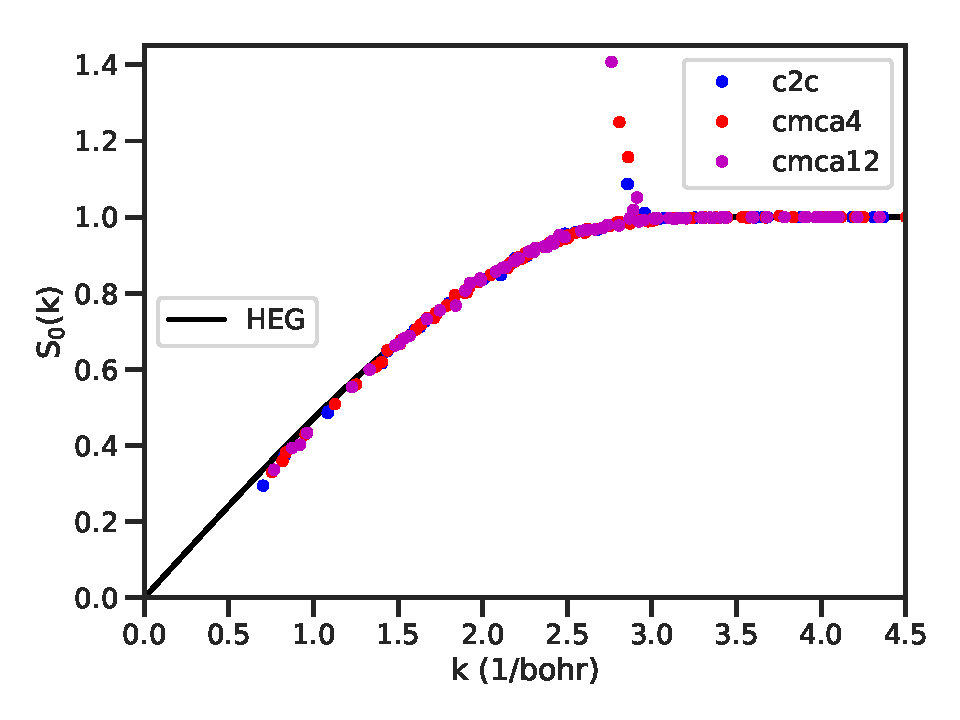
\includegraphics[width=\linewidth]{h117_mol-detsk-rs125}\\
(a) structure factor
\end{minipage}
\begin{minipage}{0.49\textwidth}
\centering
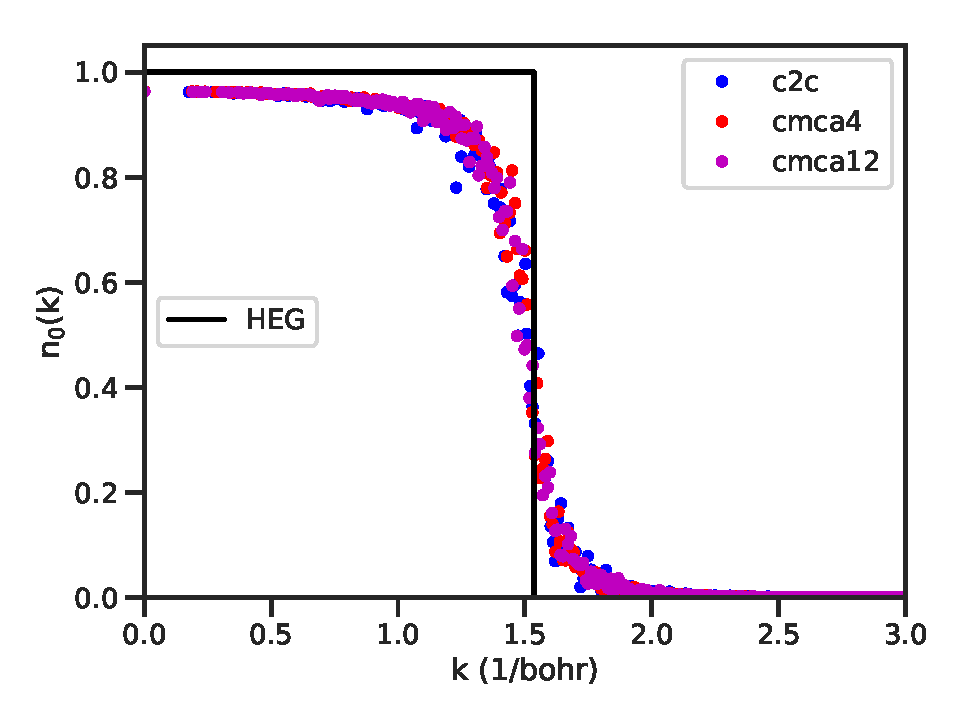
\includegraphics[width=\linewidth]{h117_mol-detnk-rs125}\\
(b) momentum distribution
\end{minipage}
\caption{Static structure factor $S_0(k)$ and momentum distribution $n_0(k)$ calculated using the Kohn-Sham determinant wave function at $r_s=1.25$. The black lines show the same functions for the free Fermi (FF) gas as reference.}
\label{fig:hsolid-det-sk-nk}
\end{figure}

The Jastrow and back flow functions are variationally optimized using the electronic hamiltonian at vdW-DF optimized clamped-ion geometries. The optimized functions at 480 GPa ($r_s\approx 1.25$) are shown in Fig.~\ref{fig:hsolid-static-jas-bf}.
These functions remain quantitatively similar across all densities explored.
The electronic components of the Jastrow and back flow functions are nearly identical for all three molecular candidates.
The largest contribution is the u-d term, which introduces correlation between unlike-spin electrons to keep them apart.
However, the electron-ion components show some variation among candidate structures, with Cmca-4 being the standout among molecular candidates.
Its optimized e-p Jastrow and back flow have much in common with those of the atomic phase.
This is likely an artifact of either the clamped-ion approximation or under-converged optimization. Once these functions are reoptimized with dynamic ions, all Jastrow and back flow components involving the electrons become essentially identical across all candidate structures, as shown in Fig.~\ref{fig:hsolid-dynamic-jas-bf}.

\begin{figure}[h]
\centering
\begin{minipage}{0.49\textwidth}
\centering
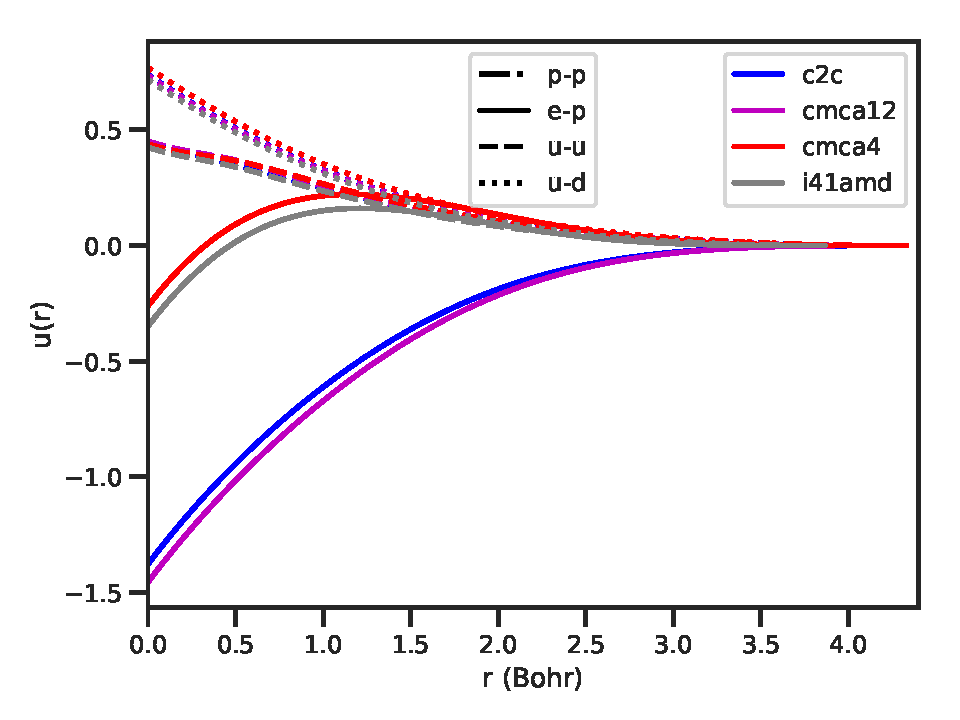
\includegraphics[width=\linewidth]{h117b_sjas-rs125}\\
(a) Jastrow pair functions
\end{minipage}
\begin{minipage}{0.49\textwidth}
\centering
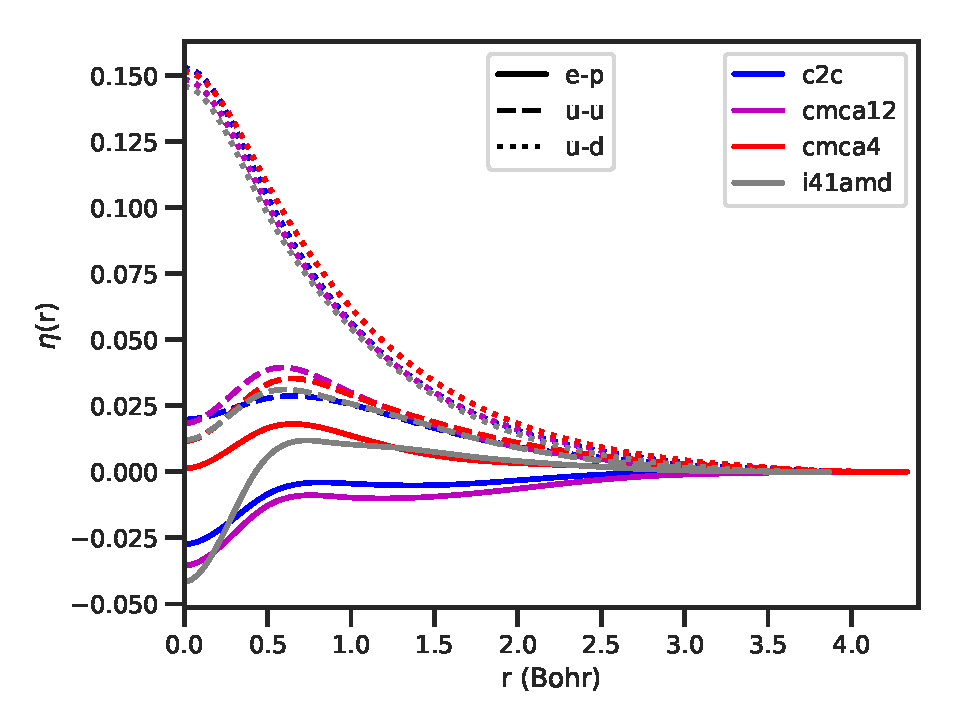
\includegraphics[width=\linewidth]{h117b_sbf-rs125}\\
(b) Back flow pair functions
\end{minipage}
\caption{Jastrow and back flow pair functions optimized at static-lattice minimum at 480 GPa. Color denotes the crystal structure. The solid line is the pair function for electron-proton, the dashed line for same-spin electrons, and the dotted lines for unlike-spin electrons.}
\label{fig:hsolid-static-jas-bf}
\end{figure}

\subsubsection{Ionic Components}
For an electron-ion simulation, the SBJ wavefunction has an additional product for distinguishable ions as well as an ion-ion Jastrow
\begin{align} \label{eq:hsolid-ei-wf}
\Psi_{ei}(\bs{R}, \bs{R}_I) = \det\left( \{ \phi_i(\bs{r}_j+\Delta\bs{r}_j; \bs{R}_I^0)\} \right) e^{-U(\bs{R},\bs{R}_I)} \prod\limits_{I=1}^{N_p} \chi(\bs{r}_I, \bs{r}_I^0),
\end{align}
where the proton orbital is an isotropic gaussian centered around its optimized geometry
\begin{align}
\chi(\bs{r}_i, \bs{r}_I^0) = \left(\dfrac{2C_p}{\pi}\right)^{3/4} \exp\left(
-C_p\vert\bs{r}_I-\bs{r}_I^0\vert
\right).
\end{align}
The expressions for the Jastrow and back flow terms remain unchanged, i.e. eq.~(\ref{eq:hsolid-ujas}) and (\ref{eq:hsolid-bf}), although the proton coordinates are now dynamic variables rather than parameters.
We take the electronic orbitals $\phi_i$ from the clamped-ion DFT calculation, performed at the vdW-DF optimized geometry, for practical purposes.
This is a severe approximation as the ideal orbitals for a system with small nonadiabatic effects should come from a Born-Oppenheimer calculation, i.e. rerun DFT at every ion position update.
Fortunately, the back flow transformation effectively changes the electronic orbitals as the ions move, because the quasi-particle position of an electron is influenced by the protons around it.

We re-optimize the Jastrow and back flow functions in dynamic-lattice VMC, using the optimized functions from static-lattice calculations as starting points.
The electron-ion Jastrow of the Cmca-4 Jastrow and back flow functions fall into good agreement with those from other candidate structures.
As shown in Fig.~\ref{fig:hsolid-dynamic-jas-bf}, after re-optimization, the only noticeable difference among the three structures lie in the proton-proton Jastrow.

\begin{figure}[h]
\centering
\begin{minipage}{0.49\textwidth}
\centering
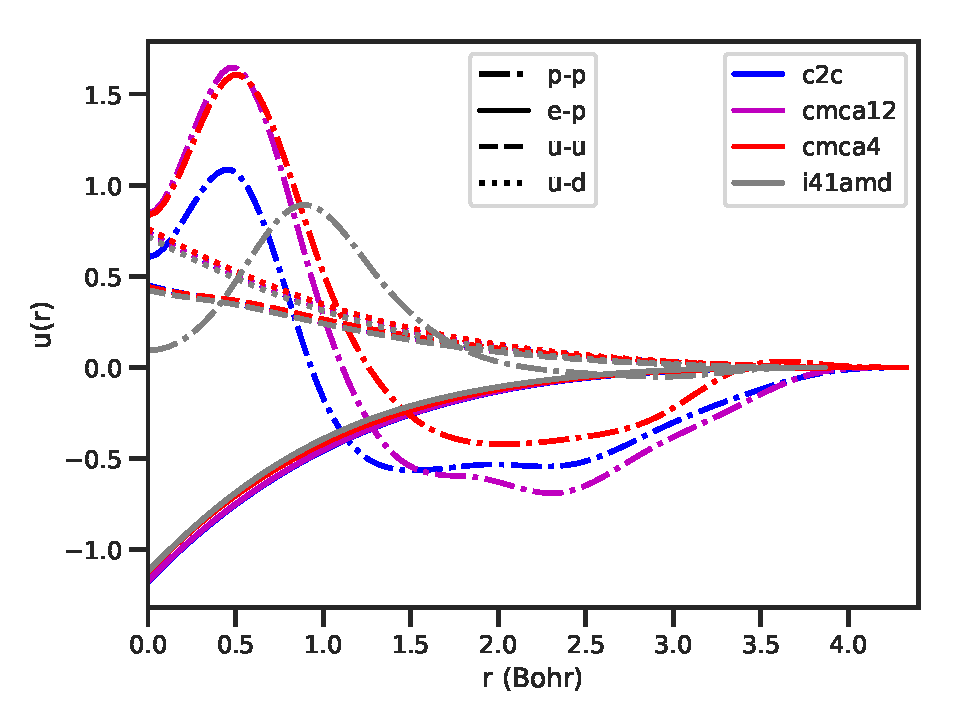
\includegraphics[width=\linewidth]{h117b_nbjas-rs125}\\
(a) Jastrow pair functions
\end{minipage}
\begin{minipage}{0.49\textwidth}
\centering
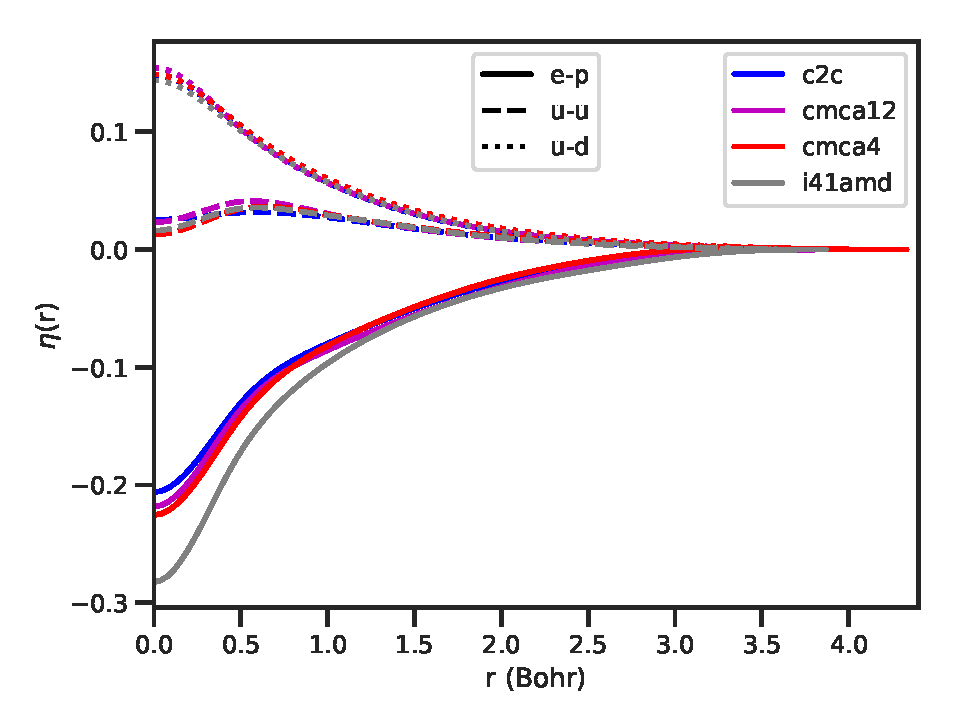
\includegraphics[width=\linewidth]{h117b_nbbf-rs125}\\
(b) Back flow pair functions
\end{minipage}
\caption{Jastrow and back flow pair functions optimized using dynamic-lattice VMC. The dash-dotted line is the pair function for proton-proton correlation. All other notations are identical to those in Fig.~\ref{fig:hsolid-static-jas-bf}.}
\label{fig:hsolid-dynamic-jas-bf}
\end{figure}

In contrast, the width of the gaussians in the proton orbital $C_p$ are optimized using \emph{maximum overlap}~\cite{Reatto1982,Natoli1993,Natoli1995}.
In this method, we measure the mean-squared deviation (MSD) of each proton from its ideal site, as determined by vdW-DF, and adjust the gaussian exponent in the proton wave function $C_p$ until the VMC and DMC estimates of the MSD agree.
This method works by maximizing the overlap between the trial and ground-state wave function along the dimension controlled by $C_p$.
Since proton MSD is a rather direct measure of the shape of the wave function and DMC pushes the VMC MSD towards its ground-state value, the optimal $C_p$ is obtained when DMC and VMC MSDs agree.
Consider an isolated proton having a normalized gaussian wave function
\begin{align}
\chi(x, y, z) = \left(\dfrac{2C_p}{\pi}\right)^{3/4} \exp\left(
-C_p(x^2+y^2+z^2)
\right).
\end{align}
The mean squared deviation of this wave function
\begin{align} \label{eq:hsolid-x2-cp}
\braket{x^2}=\braket{y^2}=\braket{z^2}=\dfrac{1}{4C_p}.
\end{align}
We expect some deviation from eq.~(\ref{eq:hsolid-x2-cp}) due to electron-proton and proton-proton correlations. When $C_p$ is large, the confining effect of the gaussian wave function dominates over correlation due to Jastrow and back-flow components, making each proton approximately independent of all other particles.
However, as $C_p$ decreases, the effects of correlation become more important. As shown in Fig.~\ref{fig:hsolid-cp-opt}(a), at large values of $C_p$ (localized protons) VMC MSDs are accurately approximated by eq.~(\ref{eq:hsolid-x2-cp}), whereas the DMC MSDs and VMC ones at small $C_p$ differ from this independent-particle approximation.
Note that the DMC runs here are short and likely under-converged.
Fortunately, they are sufficient for determining the point of maximum overlap between the VMC and DMC wave functions.
As such, the computational cost of maximum overlap optimization is more similar to VMC optimization than to a converged DMC run.
We further note that optimal $C_p$ is the same along $x$, $y$, and $z$ directions, so an isotropic Gaussian wave function is flexible enough to optimally sample the proton wave function.
Finally, the exact value of $C_p$ will not bias the DMC result so long as the projection time is sufficiently converged. This is because the protons are treated as distinguishable particles and DMC is exact at infinite projection time.

\begin{figure}[h]
\centering
\begin{minipage}{0.49\textwidth}
\centering
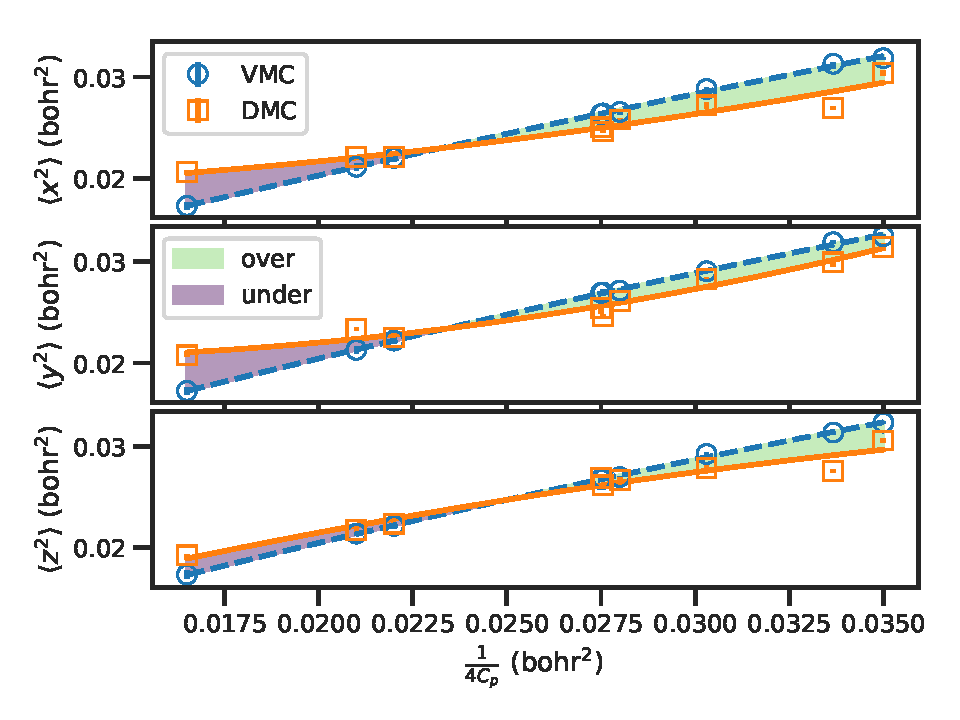
\includegraphics[width=\linewidth]{h117_copt-c2c-rs1.27-ca1.75}\\
(a) Lattice deviations vs. prediction from isolated gaussian wave function with exponent $C_p$
\end{minipage}
\begin{minipage}{0.49\textwidth}
\centering
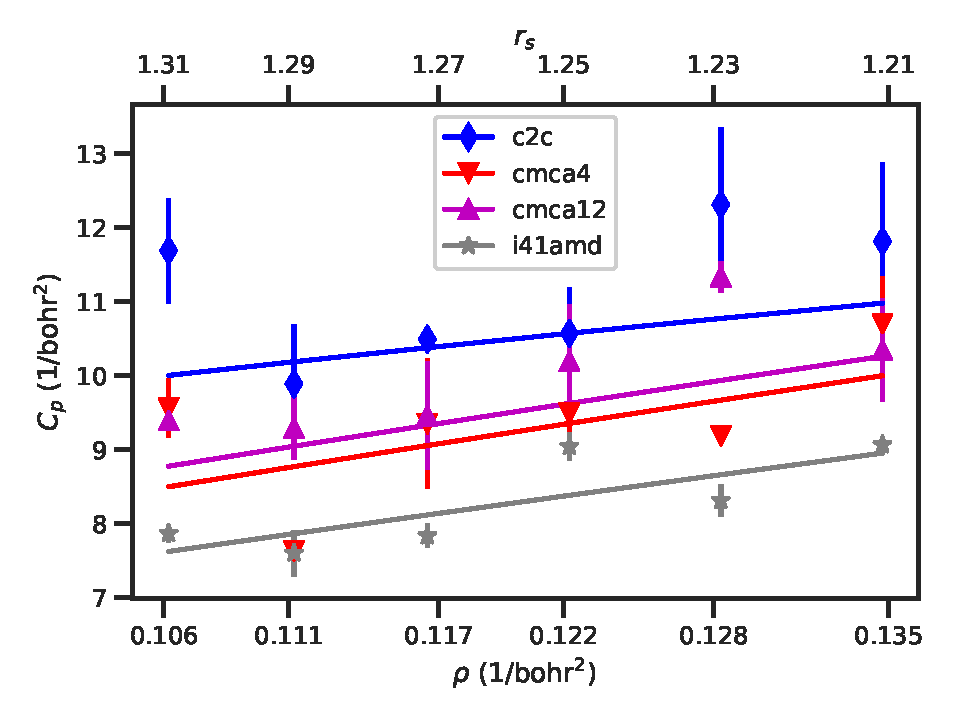
\includegraphics[width=\linewidth]{h117c_all-copt}\\
(b) optimized exponents as a function of density
\end{minipage}
\caption{Maximum overlap optimization of the proton wave function. (a) Optimization of the C2/c-24 proton wave function at $r_s=1.269$. (b) Optimized proton wave function exponent $C_p$ of all candidate structures. The markers show the $C_p$ value at the intercept of VMC and DMC. The lines are linear fits, but shifted down slightly to error on the side of oversampling. These fits are used to determine the $C_p$ value in the dynamic-lattice calculations.}
\label{fig:hsolid-cp-opt}
\end{figure}

In practice, the choice of $C_p$ is important.
Since the proton-electron mass ratio is more than $1836$, the RMSD of a proton during the diffusion process is roughly $1/43$ that of an electron in the same amount of imaginary time.
Thus, it takes more simulation time to fix errors in the proton wave function than those in the electron wave function.
Fortunately, the proton wave function is highly localized and alleviates the problem to some extend.
As shown in Fig.~\ref{fig:hsolid-cp-opt}(a), the standard deviation of the proton orbital of C2/c-24 is $<0.5$ bohr at $r_s=1.27$.
Nevertheless, it pays to choose an optimal value for $C_p$.
If $C_p$ is too large, then the proton wave function will be too localized.
This results in undersampling of the ground-state wave function and is a dangerous scenario.
During the DMC run, the kinetic energy of the protons will likely have mostly small fluctuation in this case.
However, occasional spikes, which are important for an unbiased mean will occur infrequently.
If one misses or discards these spikes, then the results will be biased.
In contrast, oversampling will increase the variance of the wave function without biasing the mean.
The resultant calculation will require more time to reach a certain accuracy target, so a balance needs to be sought.
As shown by the lines in Fig.~\ref{fig:hsolid-cp-opt}(b), we choose isotropic gaussian exponent that are close to optimal but error slightly on the side of oversampling.

\section{Results and Discussion}
\label{sec:hsolid-results}

\subsection{Static-Lattice Energy, Pressure, and Local Energy Variance}

The dominant variation of the total energy as pressure increases is due to the isotropic compression of the electron liquid and the crystal lattice. This variation is on the order of $1$ eV/p, which is roughly 50 times the energy difference among the candidate structures.
To better observe these small differences, we plot energy and pressure relative to a reference equation of state (EOS).
As a definition of zero energy at each density, this reference EOS need not be overly precise.
Nevertheless, we use a fit to high-quality DMC data for the C2/c-24 molecular crystal structure obtained by Drummond \textit{et al.}~\cite{Drummond2015}, because they are freely accessible online~\cite{drum-eos} and are well approximated by a quadratic polynomial in density.
The data file \verb|E_SJDMC_dt0_KZKcorr_v_V.dat| in directory \verb|DMC/N096/C2c-24/| contains the size-corrected DMC energy-density relation needed to fit an EOS.
As shown in Fig.~\ref{fig:hsolid-drum-eos}, we fit the high-density region of the reference data to obtain:
\begin{align}
E_0(\rho) = 1.605872\rho^2 + 0.699501\rho - 0.610902,
\label{eq:hsolid-drum-ref}
\end{align}
where $\rho=N/\Omega$ is the electron density in bohr$^{-3}$, and $E_0$ is in hartree.
We choose to fit the size-corrected 96-proton data obtained using a Slater-Jastrow wave function, because the results are easier to reproduce than its large-cell and back-flow counterparts.
The LDA-based finite-size correction scheme designed by H. Kwee, S. Zhang, and H. Krakauer (KZK)~\cite{Kwee2008} is not general in principle.
However, it was shown to work well for solid hydrogen comparing 768-proton and 96-proton results~\cite{Drummond2015}.
Equation~(\ref{eq:hsolid-drum-ref}) reproduces the QMC data to well within $1$ meV/p while interpolating between $212$ and $413$ GPa, but deviates by $1.5$ meV/p when extrapolated by $50$ GPa to $163$ GPa.
Thus, we can expect the reference EOS to be accurate over the pressure range $150$ ($r_s=1.48$) to $460$ GPa ($r_s=1.26$), but fail when extrapolated much beyond these limits.

\begin{figure}[h]
\centering
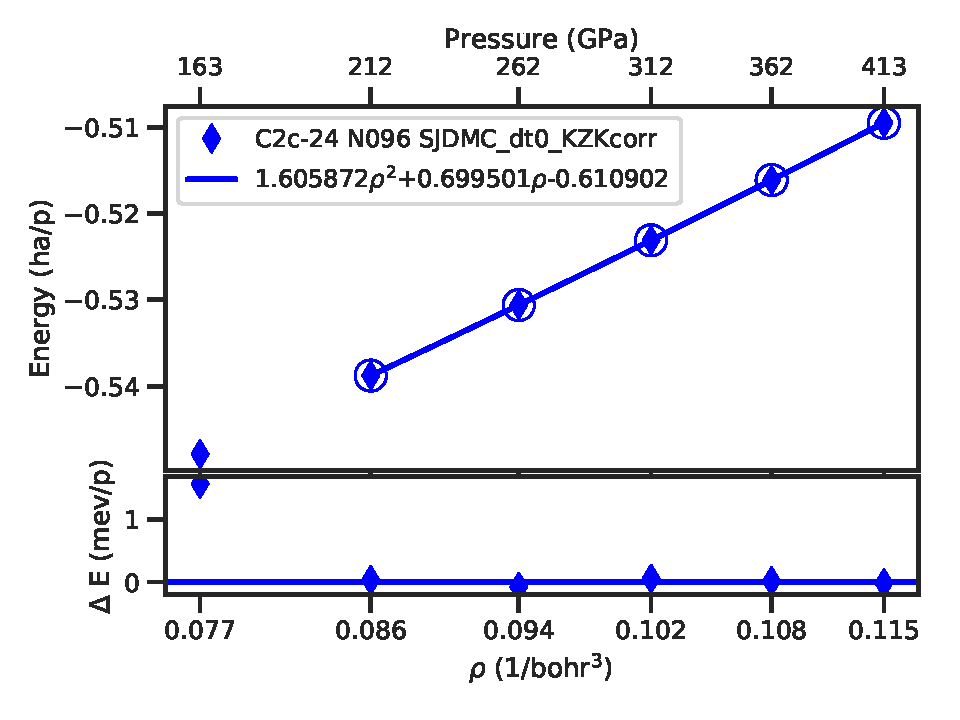
\includegraphics[scale=0.6]{h117ds_c2c-drum-eps}
\caption{Fitting of reference equation of state. The solid symbols are DMC data from Ref.~\cite{Drummond2015}, while the line is a quadratic fit to the circled points. The bottom panels shows the error in the fit.}
\label{fig:hsolid-drum-eos}
\end{figure}

The static-lattice DMC energy is plotted relative to reference in Fig.~\ref{fig:static-qmc-vs-drummond}(a). At the same density, we obtain lower total energy than Drummond \textit{et al.}~\cite{Drummond2015} partly due to our use of vdW-DF, rather than  PBE, to optimize the crystal structure; and partly due to in the inclusion of back flow transformations. At the same geometry, DMC energy is unchanged to within 3 meV/p whether PBE or vdW-DF is used to generate the orbitals in the determinant wave function.
Our C2/c curve is relatively flat at densities lower than $r_s=1.25$ and starts to bend downwards as density increases.
Thus, our C2/c pressure-density relations will be roughly identical to that of the reference EOS in the low-density region.
This is encouraging, because it implies that the fixed-node error on the pressure is small.
Even with improved geometry and wave function, we get back very similar pressure as PBE geometry and Slater-Jastrow wave function at the same density.

\begin{figure}[h]
\begin{minipage}{0.49\textwidth}
\centering
%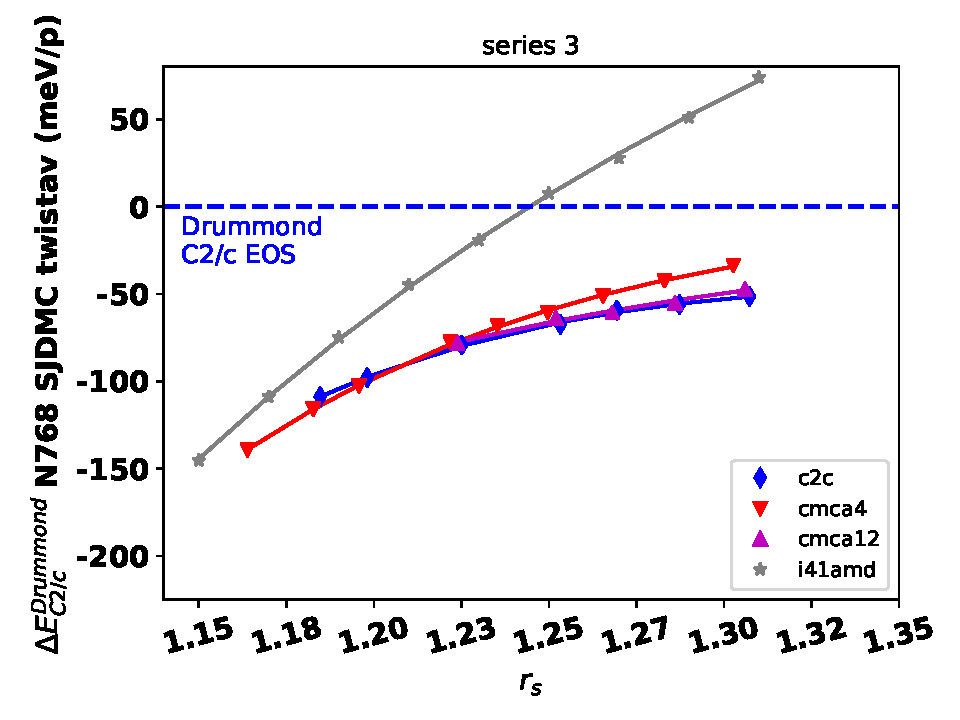
\includegraphics[width=\linewidth]{101sd_ev-s3}
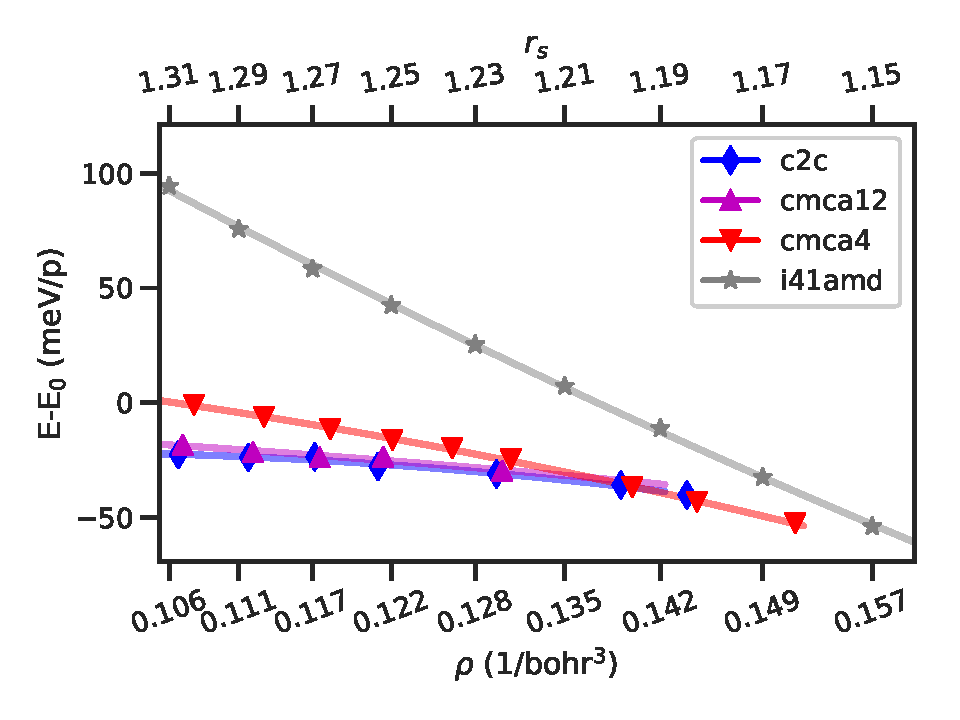
\includegraphics[width=\linewidth]{h117ds_fsc1_e-vs-rho}
(a) energy-density relation
\end{minipage}
\begin{minipage}{0.49\textwidth}
\centering
%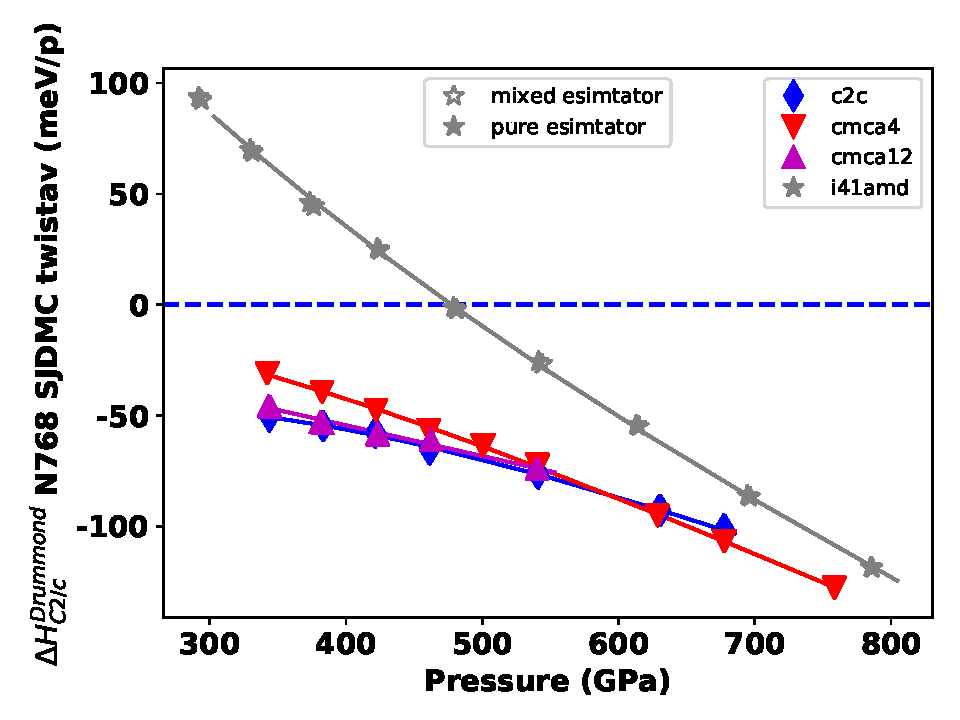
\includegraphics[width=\linewidth]{101se_hp}
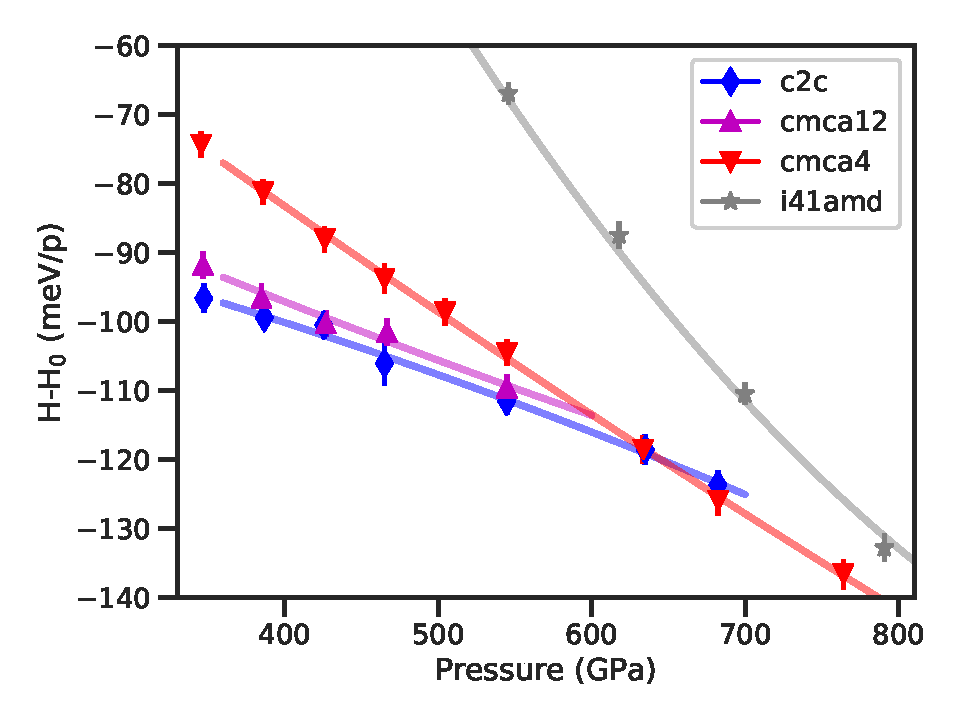
\includegraphics[width=\linewidth]{h117ds_fsc1_h-vs-p}
(b) enthalpy-pressure relation
\end{minipage}
\caption{Static-lattice DMC energy and enthalpy relative to Drummond \textit{et al.}~\cite{Drummond2015} reference eq.~(\ref{eq:hsolid-drum-ref}). Relative energies are shown in meV per proton (meV/p). Each solid line is obtained using a fitted energy-density EOS, which is obtained by fitting the finite-size corrected (FSC) total energy as a quadratic function of $\rho$. The markers are finite-size corrected simulation data without performing a fit. $P_0$ is the pressure calculated from the reference EOS $P_0=-dE_0/d\Omega$. \label{fig:static-qmc-vs-drummond}}
\end{figure}

QMC enthalpy can be calculated from virial pressure and plotted relative to the reference EOS as shown in Fig.~\ref{fig:static-qmc-vs-drummond}(b). We observe a transition from C2/c-24 to Cmca-4 around $640$ GPa and no transition to the atomic structure up to $800$ GPa.
This disagrees with the previous QMC study~\cite{McMinis2015}, showing a $450$ GPa transition from C2/c-24 to Cmca-4, which then transitions to the atomic structure around $700$ GPa.
The reason for this disagreement is unknown.

The QMC \emph{virial pressure}, calculated from kinetic energy $T$, potential energy $V$, and volume $\Omega$
\begin{align}
P = \dfrac{2T-V}{3\Omega}
\end{align}
is shown as a function of density in Fig.~\ref{fig:hsolid-p-vs-n}(a).
We first note that the QMC pressure is consistently lower than vdW-DF pressure at the same density.
Plotting the same data on a relative scale in Fig.~\ref{fig:hsolid-p-vs-n}(c),
we see that the QMC virial pressure is 4.2\% and 3.2\% lower than vdW-DF pressure at 340 GPa ($r_s\approx 1.21$) and 460 GPa ($r_s\approx 1.25$), respectively. This agrees well with the findings of R. C. Clay III \textit{et al.}, i.e. Fig.~4 in Ref.~\cite{Clay2016}.
In this plot, we also see that the mixed estimator error is 1 to 5 GPa, so the linearly-extrapolated static-lattice DMC pressure should be accurate to 1 GPa.

\begin{figure}[ht]
\centering
\begin{minipage}{0.49\linewidth}
\centering
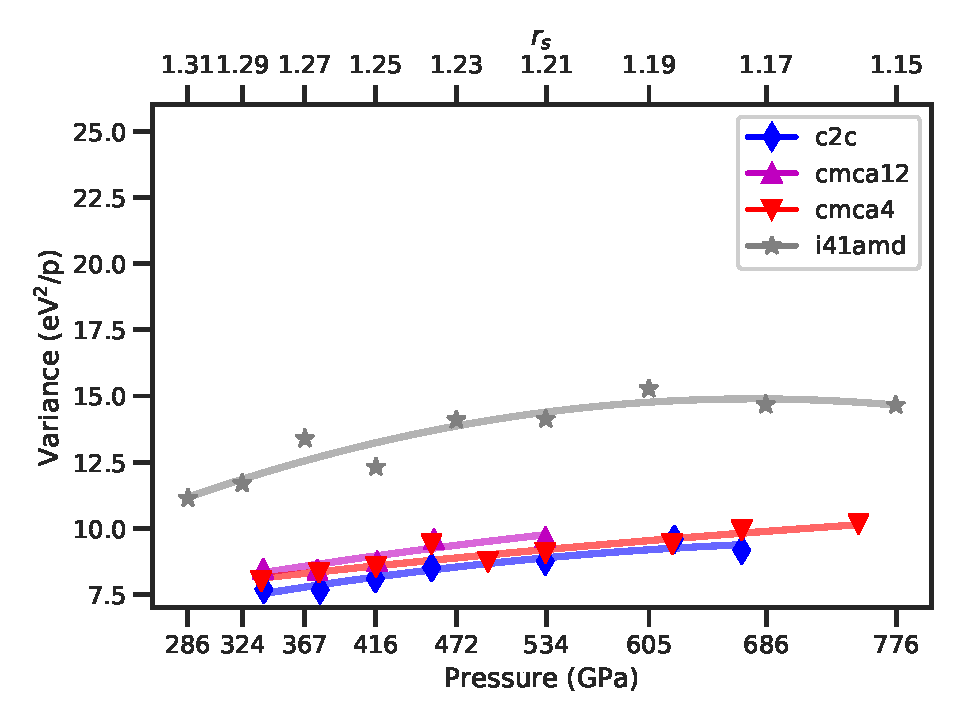
\includegraphics[width=\textwidth]{h117dc_static_var-vs-pgpa}
(a) static lattice
\end{minipage}
\centering
\begin{minipage}{0.49\linewidth}
\centering
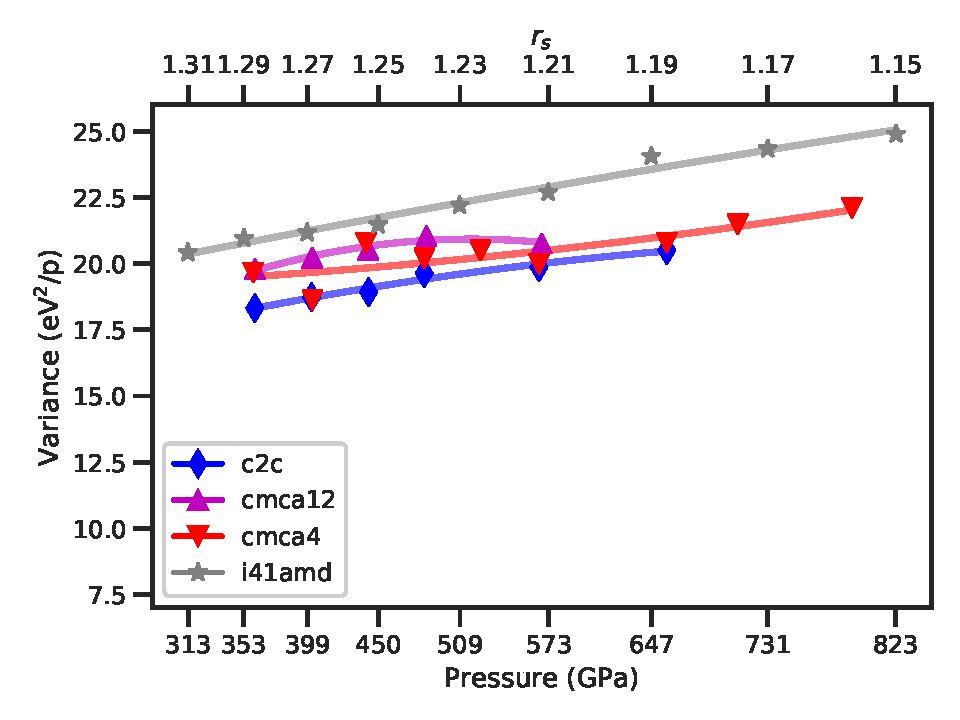
\includegraphics[width=\textwidth]{h117dc_dynamic_var-vs-pgpa}
(a) dynamic lattice
\end{minipage}
\caption{QMC variance vs. pressure. The lines are guides to the eye.}
\label{fig:hsolid-v-vs-p}
\end{figure}

Finally, the variance of the optimized static-lattice wave functions are shown in Fig.~\ref{fig:hsolid-v-vs-p}(a) as a function of pressure.
The variance of the molecular structures are $7.5\sim8.5$ eV$^2$/p below $400$ GPa and increases to $8.5\sim9.5$ eV$^2$/p at $550$ GPa.
The increase in variance may be due to the closing band gaps of the molecular structures around $400$ GPa.
If true, then it may be better to generate orbitals above $400$ GPa using the PBE functional, because it prefers metallic rather than insulating states when compared to vdW-DF.
The variance of the atomic structure is about $50$\% higher than that in the molecular phase, ranging from $11$ eV$^2$/p at $r_s=1.31$ to $15$ eV$^2$/p at high densities.
For comparison, the variance of the best analytical wave function for bcc hydrogen is $13.2(1)$ eV$^2$/p at $r_s=1.31$ (Table III in Ref.~\cite{Holzmann2003}) and $7.40(3)$ eV$^2$/p at $r_s=1.40$ (Table~2 in Ref.~\cite{Pierleoni2008}).
Small mixed-estimator error and low energy variance are hallmarks of a well-optimized wave function. We demonstrate both in Fig.~\ref{fig:hsolid-p-vs-n} and Fig.~\ref{fig:hsolid-v-vs-p} for the static-lattice electronic wave function.
The same cannot be said about the electron-ion wave function.
As shown in Fig.~\ref{fig:hsolid-v-vs-p}, the local energy variance of all structures in the dynamic-lattice calculations are twice as high as their static-lattice counterparts.
The atomic-phase variance is still roughly $3$ eV$^2$/p above the molecular structures.
This large increase in variance is due, in large part, to the use of static-lattice orbitals eq.~(\ref{eq:hsolid-ei-wf}) at all proton configurations.
They can be lowered by re-optimizing the electronic wave function upon every proton-position update, albeit at a significantly increased computational cost.

\subsection{Effect of Dynamic Ions on Energy and Pressure}
\label{sec:hsolid-dep}

When clamped protons are allowed to move, the energy of the electron-ion system changes in two ways.
First, proton kinetic energy contributes a sizable positive term to the total kinetic energy of the system. As shown in Fig.~\ref{fig:hsolid-ion-energy}(d), the kinetic energy of the protons increases from $\sim 230$ meV/p at $360$ GPa ($r_s\approx 1.31$) to $\sim 265$ meV/p at $600$ GPa ($r_s\approx 1.20$), increasing by roughly $7.3$ meV/p every $50$ GPa.
Second, the electronic wave function changes as the protons move. Thus, the electronic potential and kinetic energies change as well.
As shown in Fig.~\ref{fig:hsolid-ion-energy}(b) and (c), the increase of the total potential energy is roughly twice that of the electron kinetic energy, which is around $80\pm20$ meV/p for all candidate structures.
Unlike the increase of proton kinetic energy, the electron kinetic and total potential increases are insensitive to the electron density.
The increase of electron kinetic energy for C2/c-24 and i4$_1$/amd is $\sim 20$ meV/p higher than that of the Cmca structures, while the increase in their potential energies is $\sim 40$ meV/p lower.
The sum of all three contributions make up the total energy change from static- to dynamic-lattice, i.e. the zero-point energy (ZPE).
As shown in Fig.~\ref{fig:hsolid-ion-energy}(a), the ZPE increases from $\sim 470$ meV/p at $360$ GPa to $\sim 510$ meV/p at $600$ GPa, i.e. $8.3$ meV/p every $50$ GPa.
Most of the density dependence of the ZPE comes from the proton kinetic energy.

\begin{figure}[h]
\centering
\begin{minipage}{0.49\textwidth}
\centering
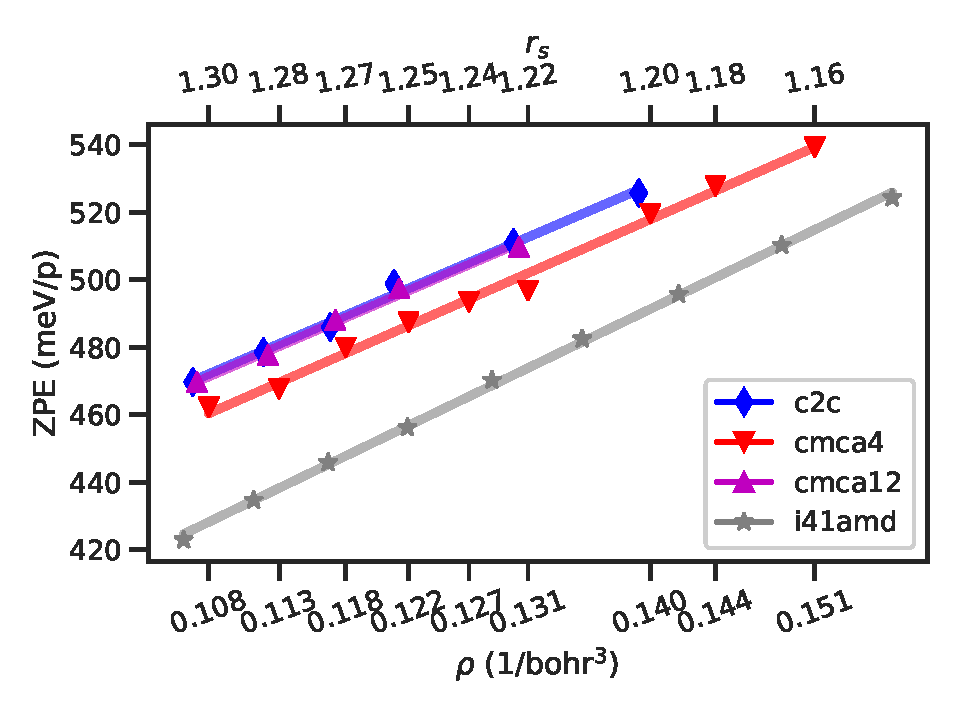
\includegraphics[width=\linewidth]{h117dc_LocalEnergy}\\
(a) total energy change (zero-point energy)
\end{minipage}
\begin{minipage}{0.49\textwidth}
\centering
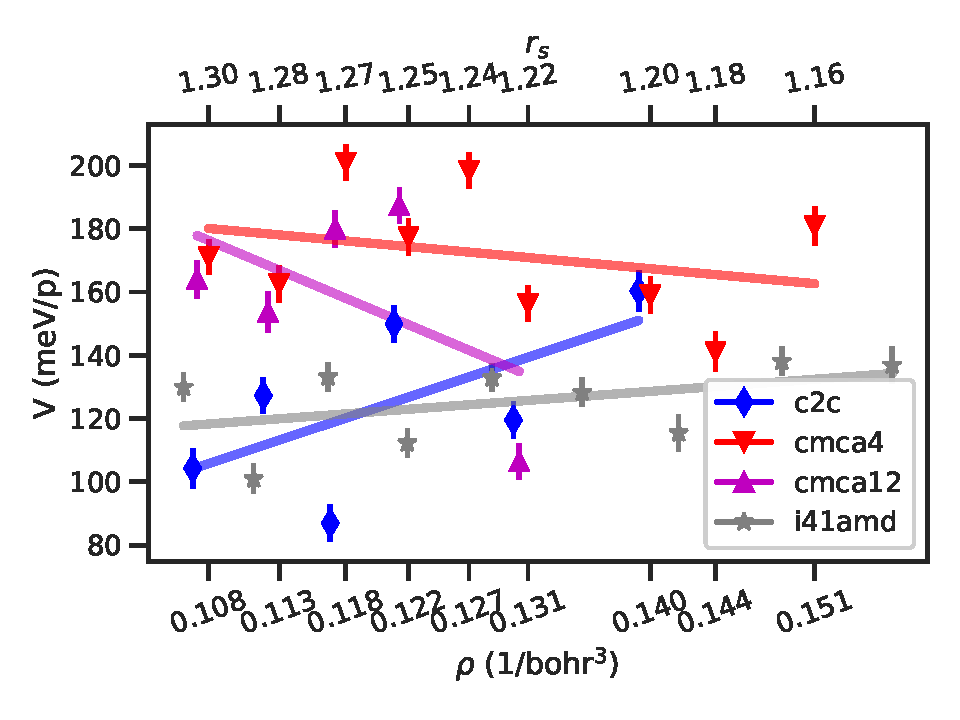
\includegraphics[width=\linewidth]{h117dc_LocalPotential}\\
(b) potential energy change
\end{minipage}
\begin{minipage}{0.49\textwidth}
\centering
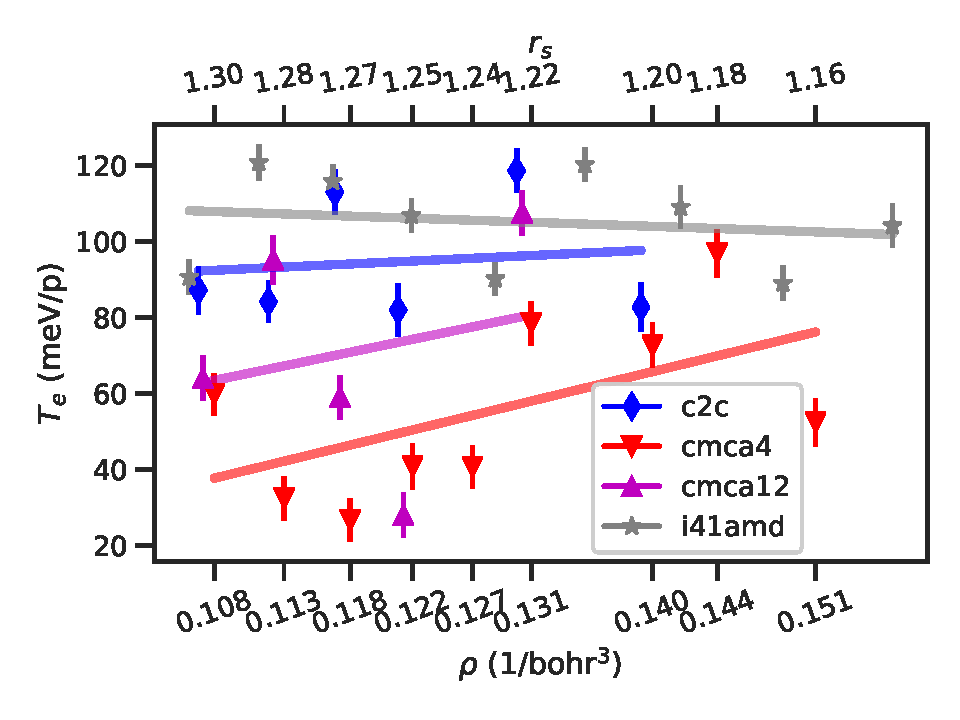
\includegraphics[width=\linewidth]{h117dc_skinetic_e}\\
(c) electronic kinetic energy change
\end{minipage}
\begin{minipage}{0.49\textwidth}
\centering
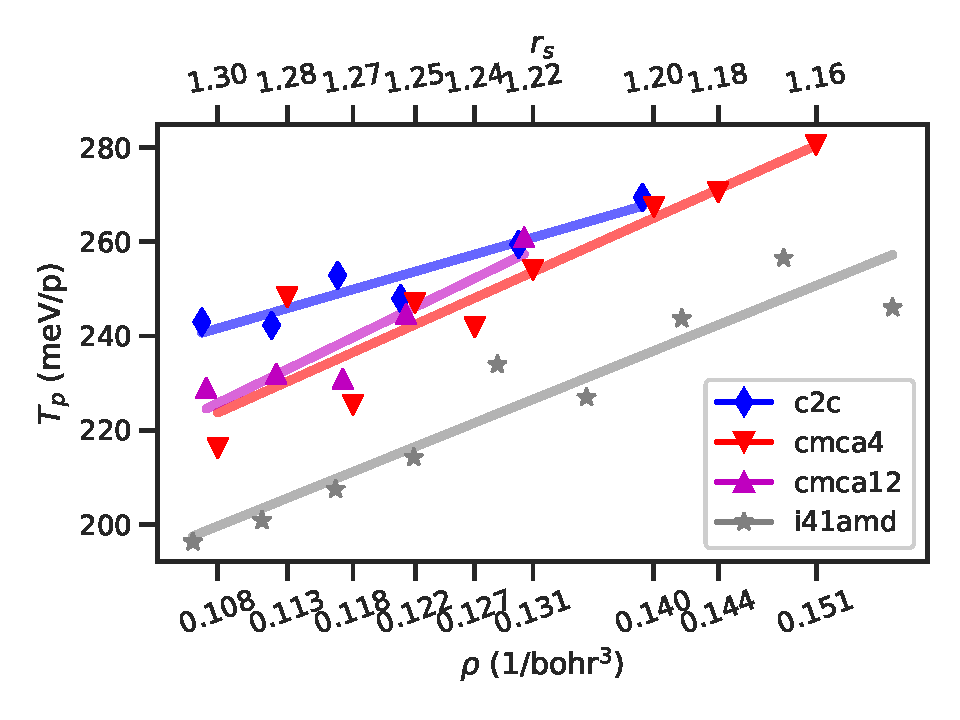
\includegraphics[width=\linewidth]{h117dc_skinetic_p}\\
(d) proton kinetic energy
\end{minipage}
\caption{Energy changes from static-lattice to dynamic-lattice simulations as functions of electron density $\rho=N/\Omega$. (a) zero-point energies of the candidate structures. (b) total potential energy change due to dynamic protons. (c) electronic kinetic energy change due to dynamic protons. (d) proton kinetic energy. Color and marker label candidate structures. The solid lines are guides to the eyes.}
\label{fig:hsolid-ion-energy}
\end{figure}

An immediate consequence of the higher kinetic and potentials energies in the dynamic-lattice simulation is higher virial pressure, about $20$ GPa higher than its static-lattice counterpart.
Interestingly, this brings the dynamic-lattice QMC pressures into better agreement with static-lattice vdW-DF pressures, as we saw in Fig.~\ref{fig:hsolid-p-vs-n} that the static-lattice QMC pressures are systematically lower by $\sim 15$ GPa.

The energy-density and enthalpy-pressure relations from the dynamic-lattice simulations are shown relative to the same reference EOS eq.~\ref{eq:hsolid-drum-ref} in Fig.\ref{fig:dynamic-qmc-vs-drummond}.
Figure~\ref{fig:dynamic-qmc-vs-drummond}(a) shows the total energy as a function of density.
First, due to ZPE, the window of energy is shifted up by roughly $500$ meV/p from its static-lattice counterpart Fig.~\ref{fig:static-qmc-vs-drummond}(a).
Second, the relative energy among molecular structures remain similar.
The C2/c-24 and Cmca-12 structures remain almost degenerate at all densities, whereas the Cmca-4 transitions from being $20$ meV/p higher in energy at $r_s=1.31$ to being the lowest-energy structure at sufficiently high density.
The transition density for Cmca-4 does decrease significantly, from $r_s=1.19$ in the static-lattice case to $r_s=1.25$ when ZPE is included.
In contrast, the overall trend of the molecular-phase total energy is noticeably changed by the inclusion of ZPE.
Instead of staying flat relative to the reference EOS, the dynamic-lattice energies of the molecular structures all trend upwards.
%This indicates that proton zero-point motion destabilizes the molecular phase more at high density than it does at low density.
Similar effects can be observed in the atomic-phase energy-density relation, although the overall upward shift due to ZPE is about $40$ meV/p less.
In summary, ZPE stabilizes the atomic phase by roughly $40$ meV/p and the Cmca-4 phase by $10$ meV/p relative the C2/c-24 and Cmca-12 without changing the relative angles at which their EOSs cross.

% exclude Cmca-4 rs=1.22
\begin{figure}[h]
\begin{minipage}{0.49\textwidth}
\centering
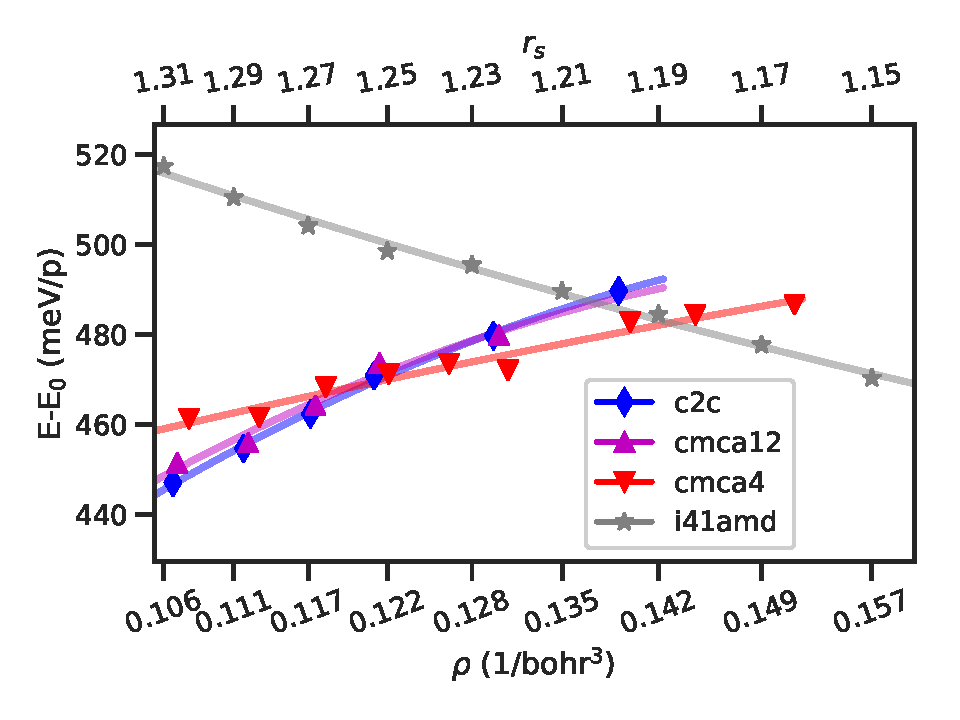
\includegraphics[width=\linewidth]{h117dd_e-vs-rho}
(a) energy-density relation
\end{minipage}
\begin{minipage}{0.49\textwidth}
\centering
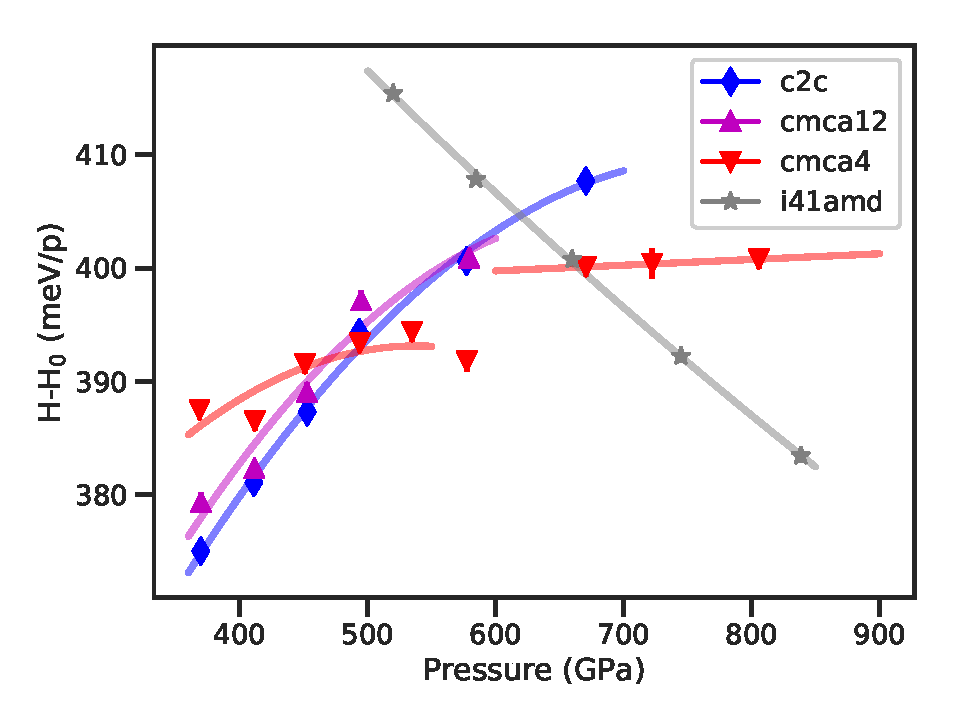
\includegraphics[width=\linewidth]{h117dd_h-vs-p}
(a) enthalpy-pressure relation
\end{minipage}
\caption{Dynamic-lattice energy and enthalpy relative to reference. Lines are quadratic fits. The crossed out points are excluded from the fit.}
\label{fig:dynamic-qmc-vs-drummond}
\end{figure}

The enthalpy-pressure relation in Fig.~\ref{fig:dynamic-qmc-vs-drummond}(b) tells the same story and we can read off the transition pressures among the candidate structures.
We see a transition from C2/c-24 to Cmca-4 slightly below 500 GPa, then a molecular-to-atomic transition around 660 GPa from Cmca-4 to I4$_1$/amd.
The calculated transition pressure to the atomic phase is $160$ GPa higher than the previous QMC calculation~\cite{McMinis2015} and a reported experimental observation~\cite{Silvera2017}.
However, the previous calculation used the harmonic approximation to calculate proton ZPE, while the experiment made little characterization of the final sample and has yet to be reproduced.
As such, a $660$ GPa transition pressure is not outside the realm of possibilities.
Admittedly, the current approach has its own drawbacks.
The most concerning approximation is the use of static-lattice orbitals in the electron-ion wave function eq.~(\ref{eq:hsolid-ei-wf}).
%h5ca/frozen_dE_vs_r.eps
This ``frozen orbital'' approach incurs around $80$ meV/p more fixed-node error than a Born-Oppenheimer wave function fully-optimized at each new geometry, although this error cancels well between molecular and atomic phases.

\subsection{Effect of Dynamic Ions on Electronic Correlation Functions}

\begin{figure}[h]
\centering
\begin{minipage}{0.49\textwidth}
\centering
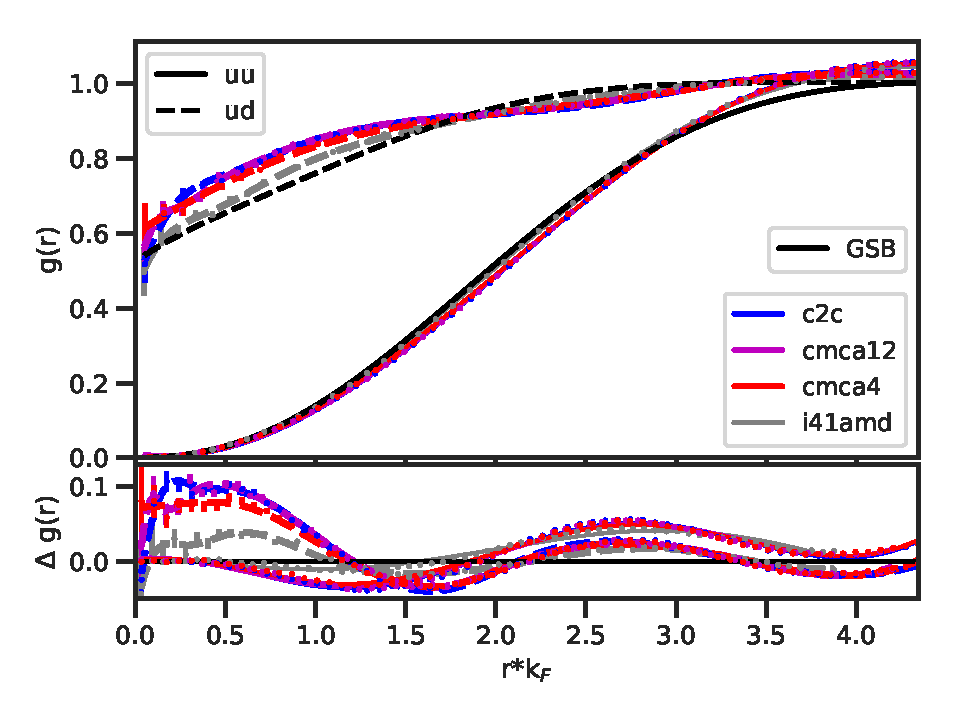
\includegraphics[width=\linewidth]{h117ga_static-rs125-s2-gr}\\
(a) static lattice
\end{minipage}
%\begin{minipage}{0.49\textwidth}
%\centering
%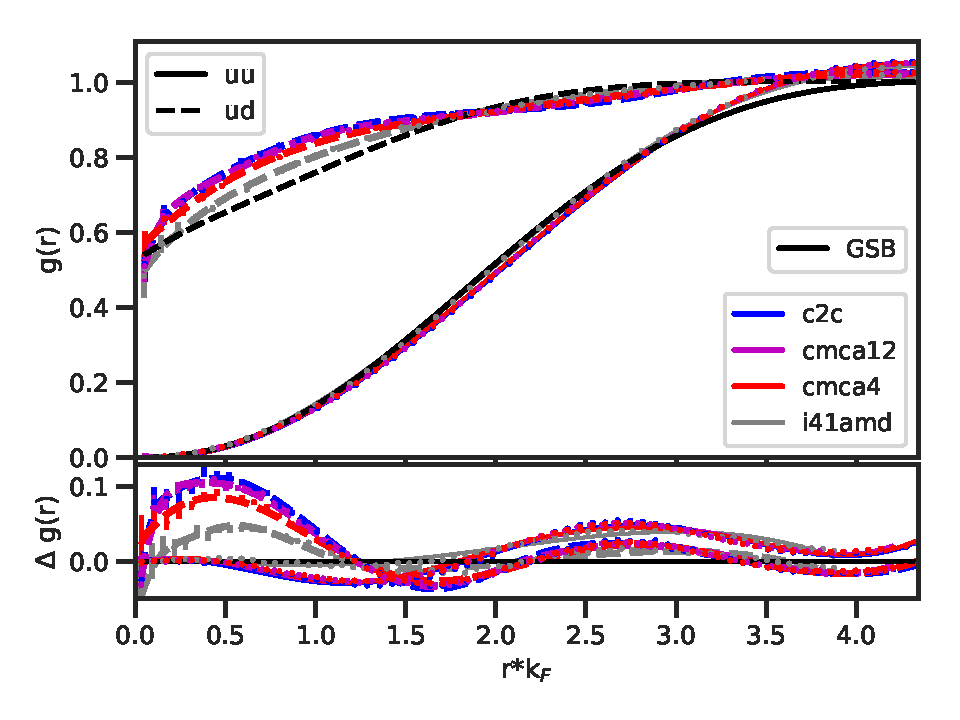
\includegraphics[width=\linewidth]{h117ga_dynamic-rs125-s0-gr}\\
%(b) dynamic lattice VMC
%\end{minipage}
\begin{minipage}{0.49\textwidth}
\centering
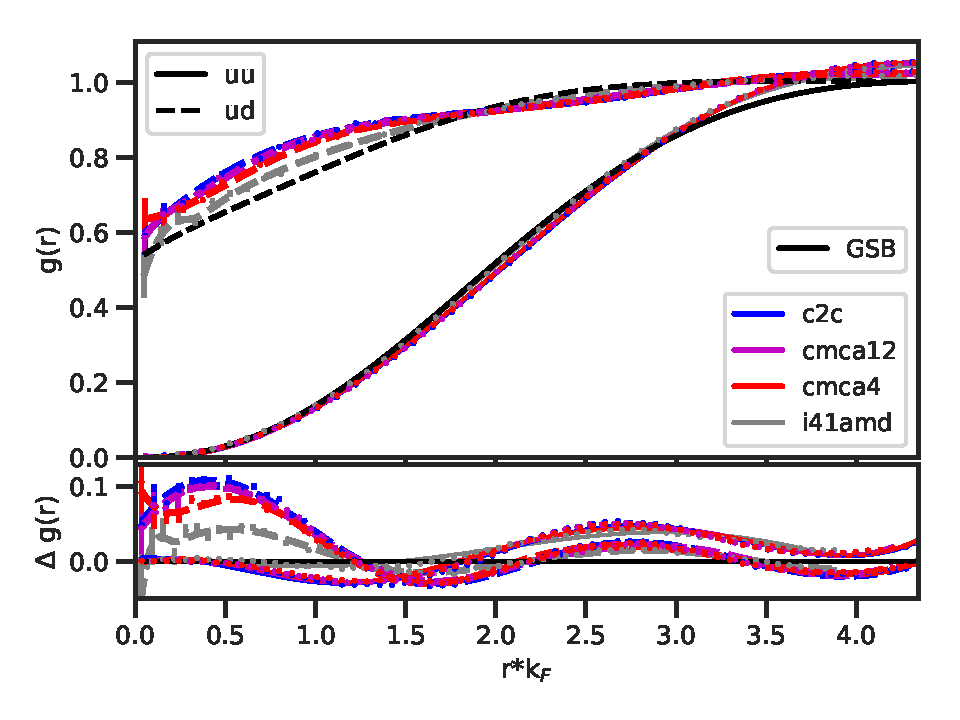
\includegraphics[width=\linewidth]{h117ga_dynamic-rs125-s2-gr}\\
(b) dynamic lattice %DMC ts=3.0
\end{minipage}
%\begin{minipage}{0.49\textwidth}
%\centering
%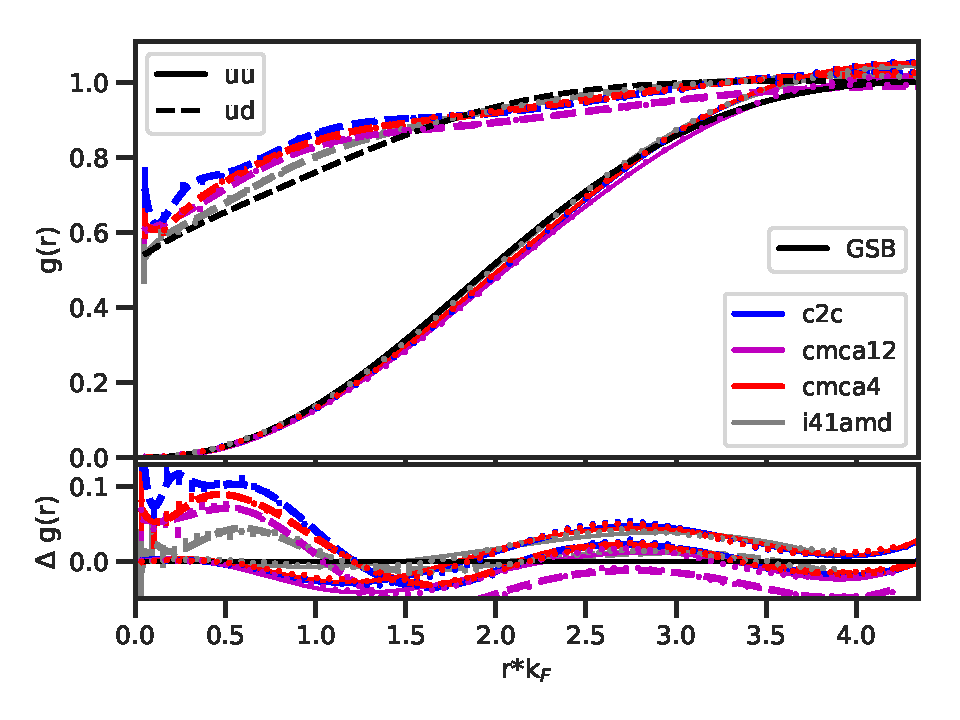
\includegraphics[width=\linewidth]{h117ga_dynamic-rs125-s3-gr}\\
%(d) dynamic lattice DMC ts=1.5
%\end{minipage}
\caption{DMC electronic pair correlation functions at $r_s=1.25$. Color denotes candidate structure, while the black lines are $g(r)$ of the unpolarized homogeneous electron gas at the same density as parametrized by P. Gori-Giorgi, F. Sacchetti and G. B. Bachelet (GSB)~\cite{Gori-Giorgi2000}.}
\label{fig:hsolid-eegr}
\end{figure}

The electron-electron pair correlation function are shown in real space $g(r)$ in Fig.~\ref{fig:hsolid-eegr}.
The correlation functions of the 3D unpolarized homogeneous electron gas are also shown as reference.
The bottom panel of each plot shows the difference between the hydrogen $g(r)$s from those of the electron gas.
This difference highlights the modification of the electron liquid due to the ionic lattice.
The dynamic-lattice electronic $g(r)$s are identical to those from the static-lattice calculations on the scale of the difference panel ($0.1$).
For the molecular structures, both the same-spin (u-u) and unlike-spin (u-d) $g(r)$s are the same over the entire range from zero ($r=0$) to the supercell image distance ($r=R_{WS}$).
The most notable deviation from the electron gas is an enhanced correlation between unlike-spin electrons at small separation.
This is likely due to the presence of covalent bonds, formed by a pair of unlike-spin electrons at the center of each H$_2$ molecules.
A more subtle difference is the presence of small periodic modulations of the electronic $g(r)$ that seem to persist to long distances.
The atomic structure shows no enhancement of unlike-spin correlation function at $r=0$, whereas it shows the same periodic modulations as the molecular structures at long range.

\begin{figure}[h]
\centering
\begin{minipage}{0.49\textwidth}
\centering
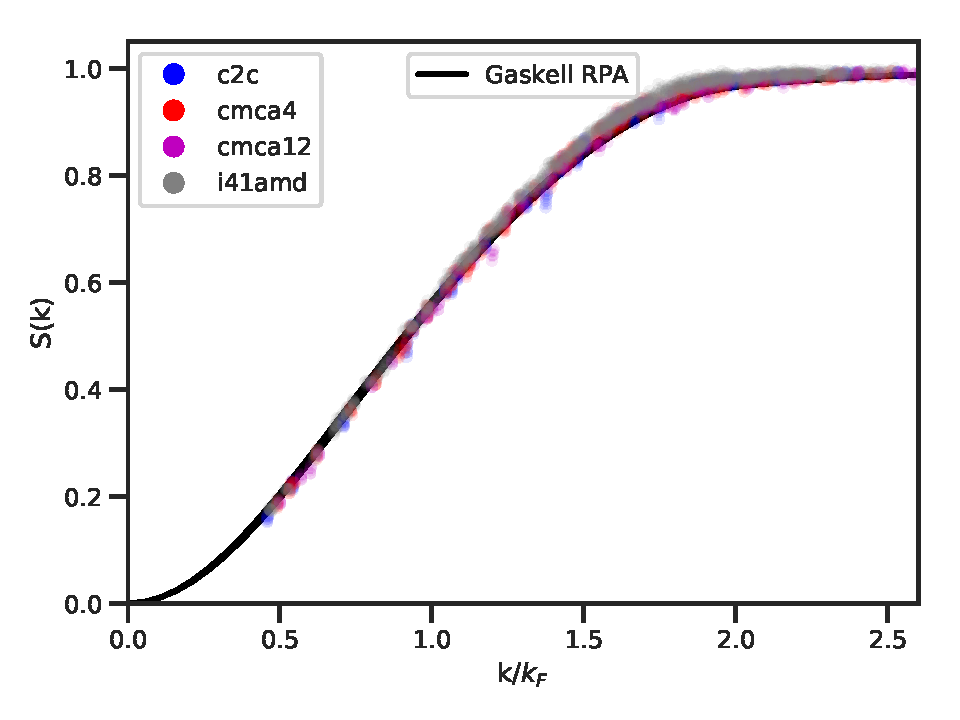
\includegraphics[width=\linewidth]{h117_grsk-static-sk}\\
(a) static
\end{minipage}
\begin{minipage}{0.49\textwidth}
\centering
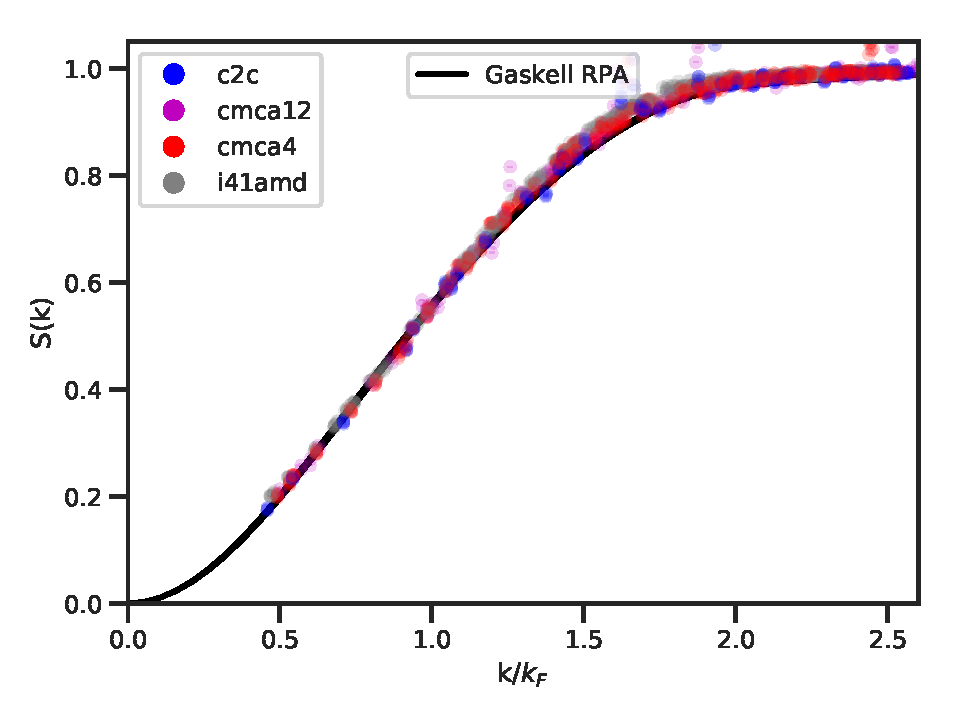
\includegraphics[width=\linewidth]{h117_grsk-dynamic-esk}\\
(b) dynamic
\end{minipage}
\caption{Electron-electron static structure factor $S(k)$.}
\label{fig:hsolid-esk}
\end{figure}

The electron-electron static structure factor is shown in Fig.~\ref{fig:hsolid-esk}.
At all densities and for all structures, both static-lattice and dynamic-lattice results are in excellent agreement with RPA $S(k)$ for the electron gas.
However, small increase in correlation can be seen at intermediate range $k/k_F\approx 1.5$.
Further, subtle differences at long-range ($k\rightarrow0$) can make the electronic properties of the candidate structures qualitatively different from those of the electron gas and from each other.

\begin{figure}[h]
\centering
\begin{minipage}{0.49\textwidth}
\centering
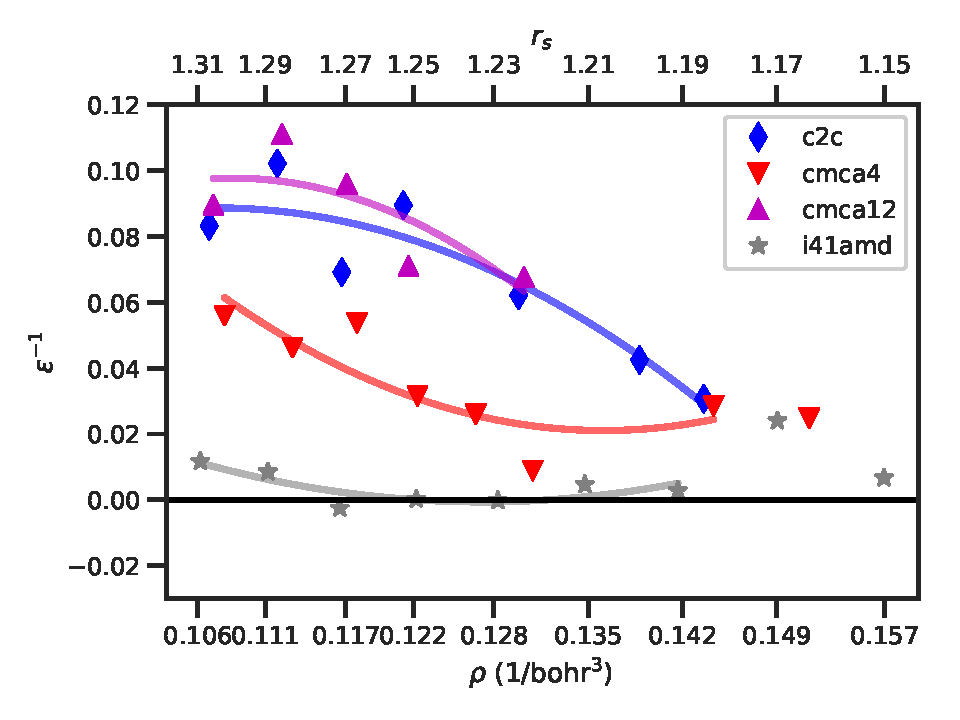
\includegraphics[width=\linewidth]{h117gs_eps-vs-rho}\\
(a) static lattice
\end{minipage}
\begin{minipage}{0.49\textwidth}
\centering
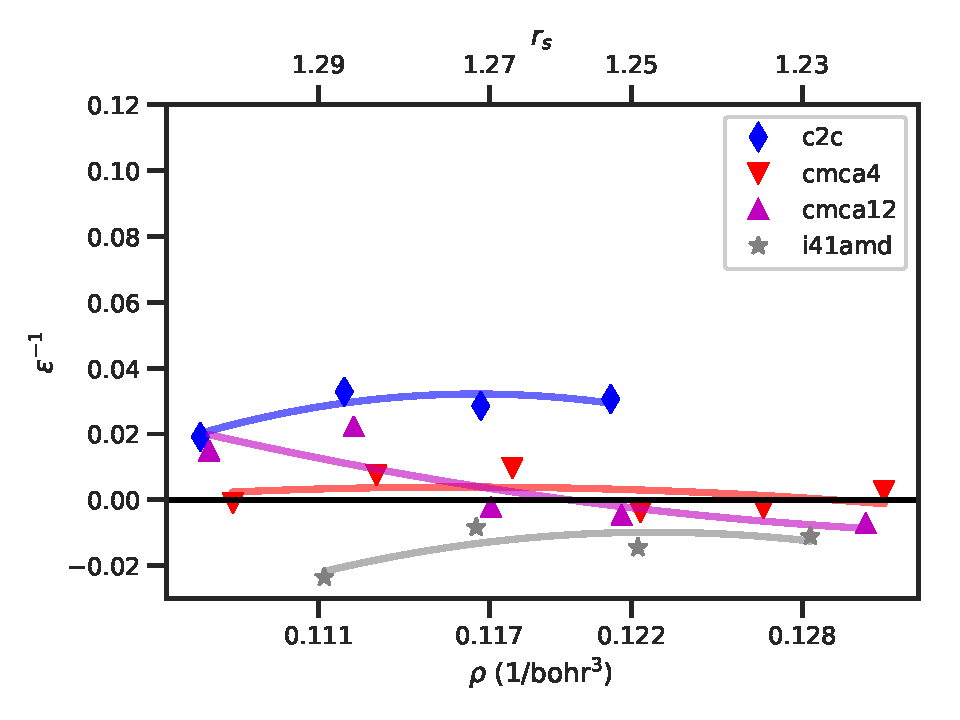
\includegraphics[width=\linewidth]{h117gd_eps-vs-rho}\\
(b) dynamic lattice
\end{minipage}
\caption{Upper bound on inverse dielectric constant.}
\label{fig:hsolid-epsinv}
\end{figure}

%\subsection{Dielectric Constants from S(k)}
The inverse dielectric function is bounded from above by $\epsilon^{-1}(\bs{k}) \le 1-\Gamma_{\bs{k}}^2$, where
\begin{align}
\Gamma_{\bs{k}} = \dfrac{2m S(\bs{k})}{\hbar^2 \bs{k}^2}.
\end{align}
The limit $\lim\limits_{k\rightarrow0} 1-\Gamma_k^2$ can be a good approximation to the inverse dielectric constant of an isotropic system.
The inequality becomes an equality if there is only a single excitation energy such as a plasmon at long wavelength.
Importantly, if this limit reaches zero, then the material is metallic.
In Fig.~\ref{fig:hsolid-epsinv}, the isotropic limit is shown as a function of density.
There are sizable systematic errors in these results due to a lack of data at small $k$ and the choice of fitting range.
These systematic errors are not precisely estimated, but its size should be comparable to the oscillation of the data points.
The inaccessible region around $\bs{k}=\bs{0}$ increases with density, so the high-density results are less reliable than the low-density ones.
In the static-lattice results Fig.~\ref{fig:hsolid-epsinv}(a), the atomic structure is metallic at all densities as expected.
The Cmca-4 and C2/c-24 structures become metallic at roughly $r_s=1.22$ and $r_s=1.17$, respectively. These densities correspond to $550$ GPa and $800$ GPa, which are higher than experiment~\cite{Loubeyre2020} and calculation~\cite{Gorelov2019}.
It is possible that the molecular structures first start to conduct in-plane while being insulating across the planes.
In this case, the isotropic dielectric bound derived from spherically averaged $S(k)$ will overestimate the metalization pressure.
The dynamic-lattice results Fig.~\ref{fig:hsolid-epsinv}(b) show all structures as metallic at densities higher than $r_s=1.26$ ($460$ GPa) except for C2/c-24, which remains borderline insulating.

\subsection{Proton-proton g(r) and S(k)}

\begin{figure}[h]
\centering
\begin{minipage}{0.49\textwidth}
\centering
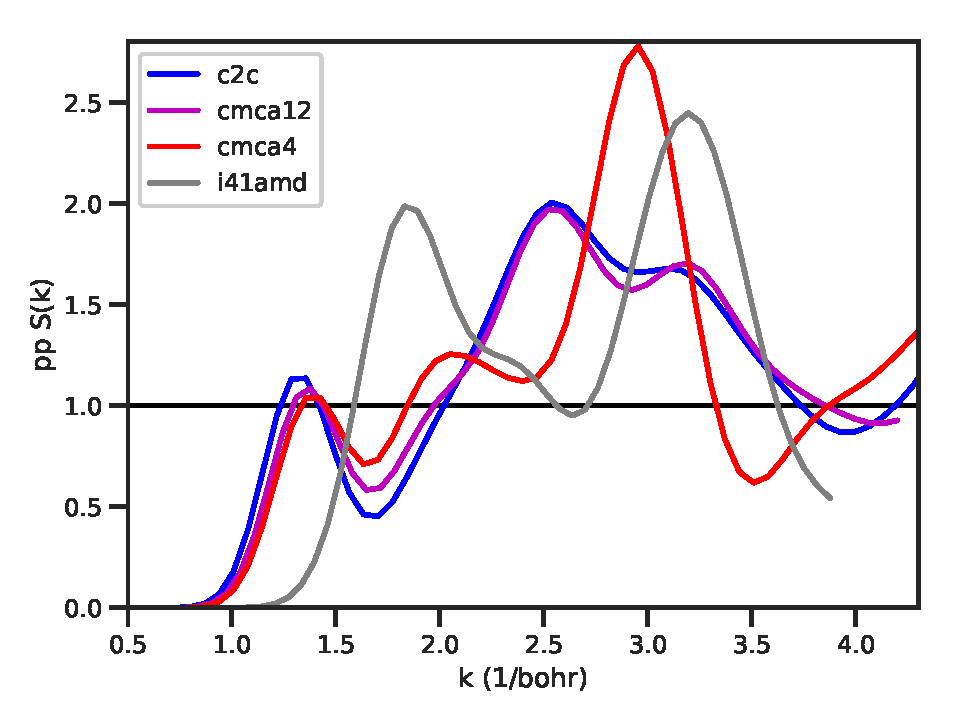
\includegraphics[width=\linewidth]{h117gd_ppgr-s2}\\
(a) pair correlation function $g(r)$
\end{minipage}
\begin{minipage}{0.49\textwidth}
\centering
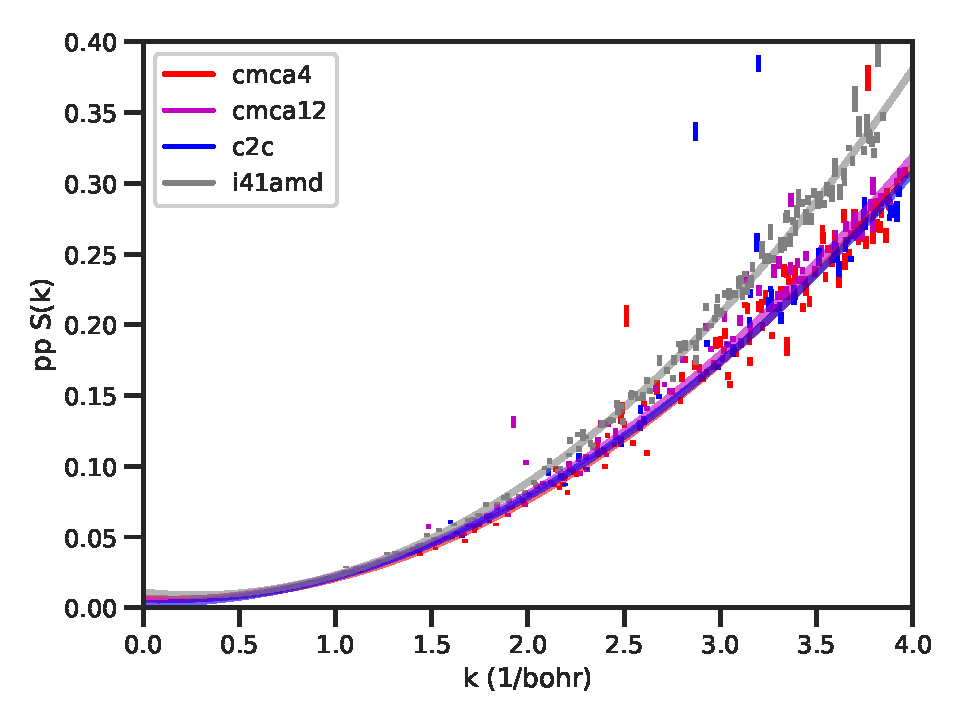
\includegraphics[width=\linewidth]{h117gd_sk0-s2}\\
(b) static structure factor $S(k)$
\end{minipage}
\centering
\begin{minipage}{0.49\textwidth}
\centering
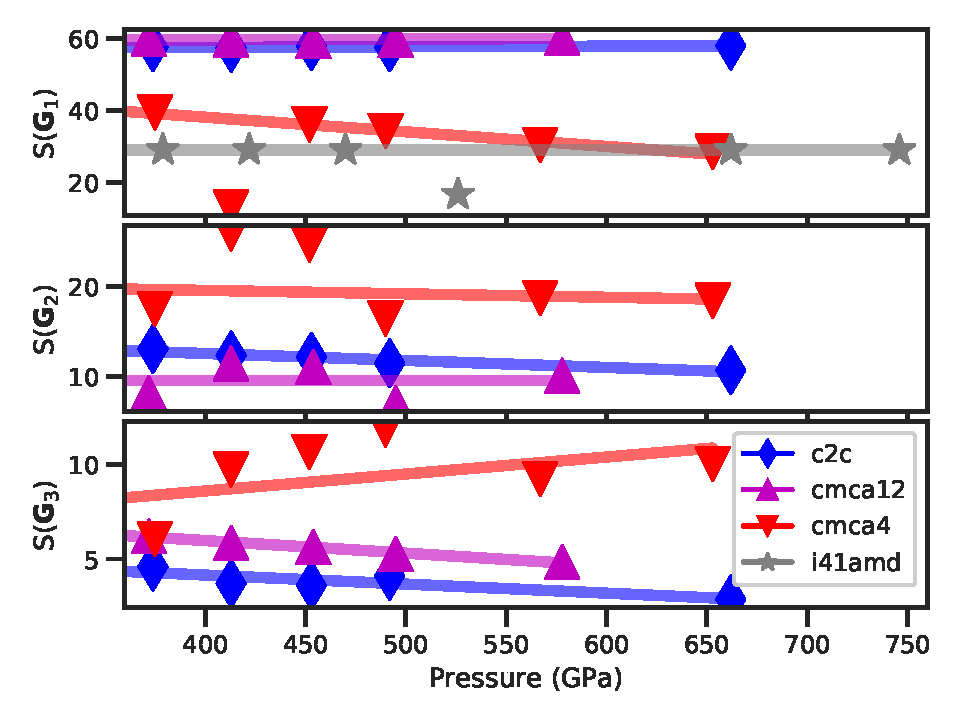
\includegraphics[width=\linewidth]{h117gd_ppsk-peaks-vs-pgpa}\\
(c) Bragg peaks of p-p $S(k)$
\end{minipage}
\begin{minipage}{0.49\textwidth}
\centering
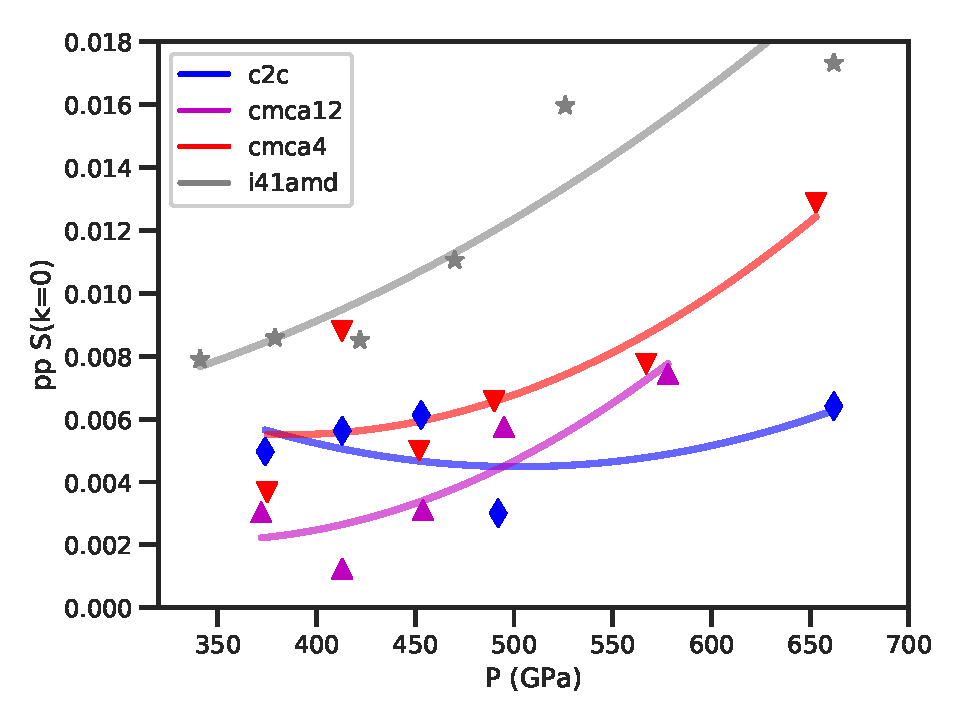
\includegraphics[width=\linewidth]{h117gd_ppsk-k0-vs-pgpa}\\
(d) long wavelength limit
\end{minipage}
\caption{Proton-proton pair correlation functions around $r_s=1.25$ ($480$ GPa). The solid lines in (b) are quadratic fits to the smooth part of $S(k)$. (c) Bragg peaks of the p-p $S(k)$ (d) long wavelength limit $S(0)$.  $\vert\bs{G}_1\vert\approx 1.81$ bohr$^{-1}$, $\vert\bs{G}_2\vert\approx 1.87$ bohr$^{-1}$ for all three molecular structures. $\vert\bs{G}_3\vert\approx 2.5$ for C2/c-24 and Cmca-4 and $1.93$ for Cmca-12. The atomic structure's Bragg peak can be found between $1.83$ and $1.88$ bohr$^{-1}$. The same outliers as Fig.~\ref{fig:dynamic-qmc-vs-drummond} are excluded from the quadratic fits in (d).}
\label{fig:hsolid-ppgrsk}
\end{figure}

The proton-proton pair correlation function of all candidate structures at $r_s\approx1.25$ are shown in Fig.~\ref{fig:hsolid-ppgrsk}(a).
Every molecular structure has a peak at the molecular bond length, in agreement with the DFT bond lengths shown in Fig.~\ref{fig:hsolid-vdw-ca}(b).
C2/c-24 bond length is around $1.35$ bohr, Cmca-4 around $1.40$ bohr, and the Cmca-12 structure is in between.
The C2/c-24 and Cmca-12 structures have remarkably similar p-p g(r).
Since they are almost degenerate over the entire density range explored, we can infer that the slight monoclinic distortions of their unit cells and the small differences in their molecular bond lengths do not contribute significantly to the total energy.
The less distorted C2/c-24 structure is more stable.
The Cmca-4 structure is significantly different from C2/c-24. Cmca-4 has second- and third-nearest neighbor peaks at $2$ and $3$ bohr, respectively, rather than C2/c-24's $2.5$ and $3.2$. The size and shape of these peaks are more similar to those in the atomic structure than the other molecular candidates.

The long-range fluctuation and order of the protons can be observed in the proton-proton static structure factor. Its fluctuating part is shown in Fig.~\ref{fig:hsolid-ppgrsk}(b).
All three molecular candidates have very similar levels of long-range fluctuations, whereas the atomic structure has noticeably more.

The molecular structures have more crystalline signatures than the atomic phase.
As shown in Fig.~\ref{fig:hsolid-ppgrsk}(c), after spherical average, each molecular structure has at least three Bragg peaks for $k<4$ bohr$^{-1}$, while the atomic structure has only one.
The C2/c-24 and Cmca-12 Bragg peaks have very similar intensities and remain relatively unchanged by pressure.
However, the Cmca-4 structure's most intense Bragg peak is comparable with that in the atomic structure and decreases in intensity as pressure increases.
Finally, the long wavelength limit of the static structure factor can be related to the isothermal compressibility $\kappa\equiv n(\dfrac{\partial P}{\partial n})\vert_T$
\begin{align}
nk_BT\kappa = S(\bs{0}),
\end{align}
where $n$ is the density. We can extract the long wavelength limit of the p-p $S(k)$ by fitting its fluctuating part to a quadratic polynomial as shown in Fig.~\ref{fig:hsolid-ppgrsk}(a).
The value of the fit extrapolated to $k=0$ is shown as a function of pressure for all candidates in Fig.~\ref{fig:hsolid-ppgrsk}(d).
The compressibility of C2/c-24 is approximately independent of pressure, whereas that of the Cmca structures and the atomic structure increase with pressure at a similar rate.
The atomic structure is twice as compressible as the molecular structures at all pressures.

\begin{figure}[h]
\centering
\begin{minipage}{0.49\textwidth}
\centering
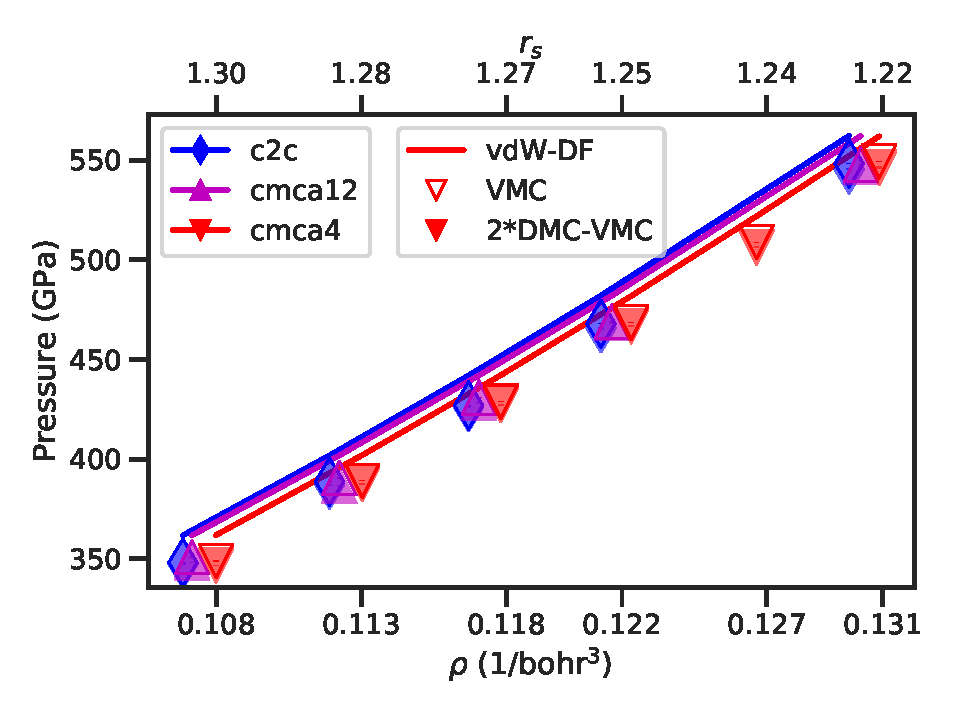
\includegraphics[width=\linewidth]{h117_evp-static-fsc1-rel0-rm121}\\
(a) static-lattice absolute scale
\end{minipage}
\begin{minipage}{0.49\textwidth}
\centering
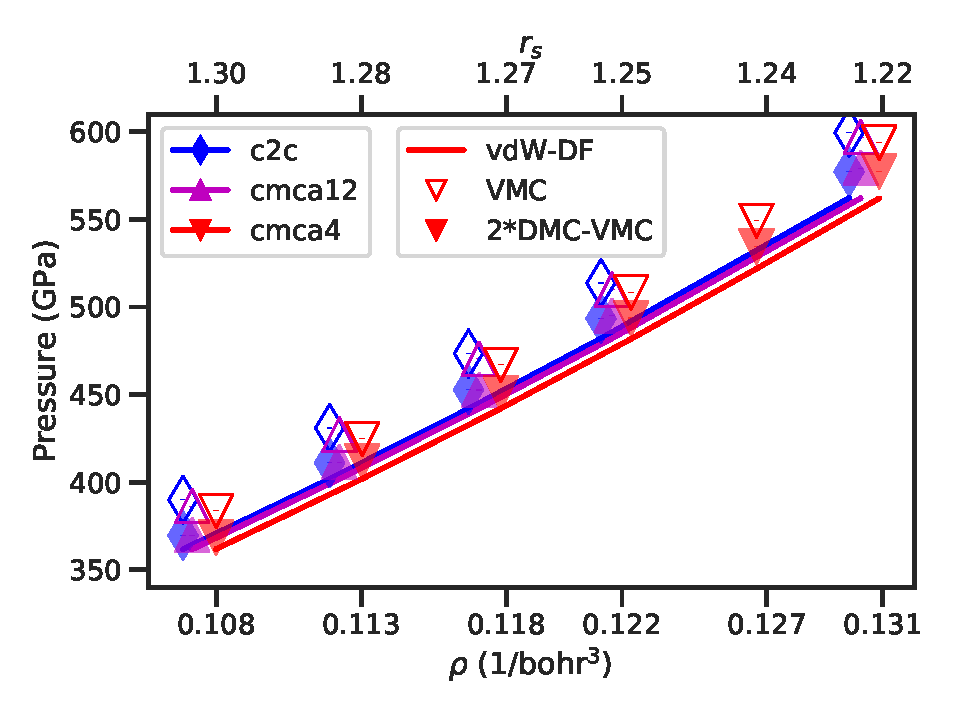
\includegraphics[width=\linewidth]{h117_evp-dynamic-fsc1-rel0-rm121_p-rs}\\
(b) dynamic-lattice absolute scale
\end{minipage}
\begin{minipage}{0.49\textwidth}
\centering
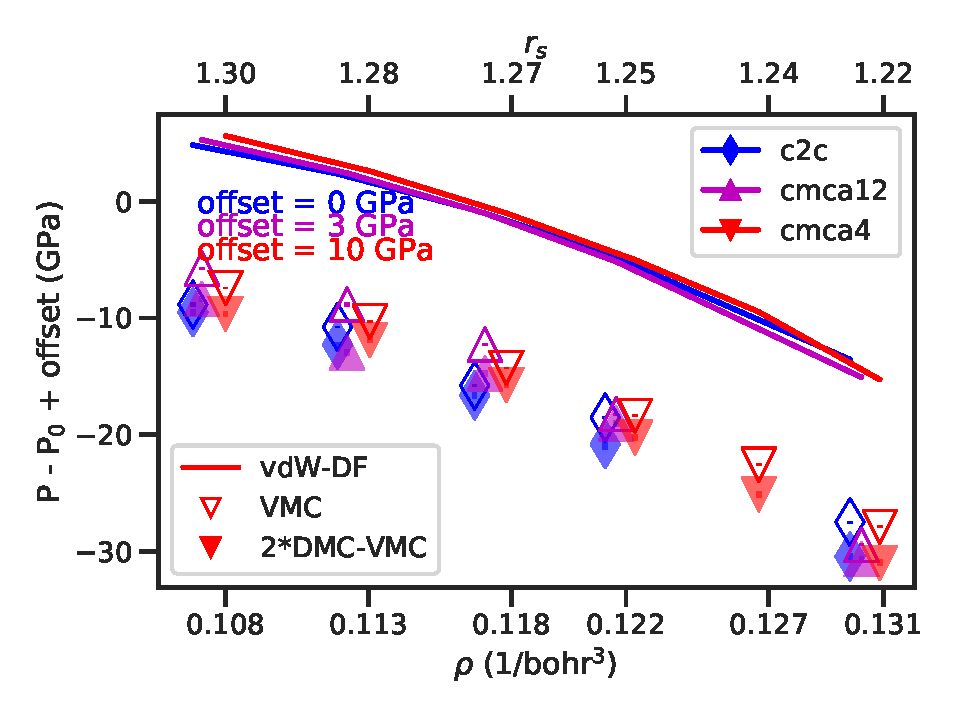
\includegraphics[width=\linewidth]{h117_evp-static-fsc1-rel1-rm121}\\
(c) static-lattice relative to $P_0$
\end{minipage}
\begin{minipage}{0.49\textwidth}
\centering
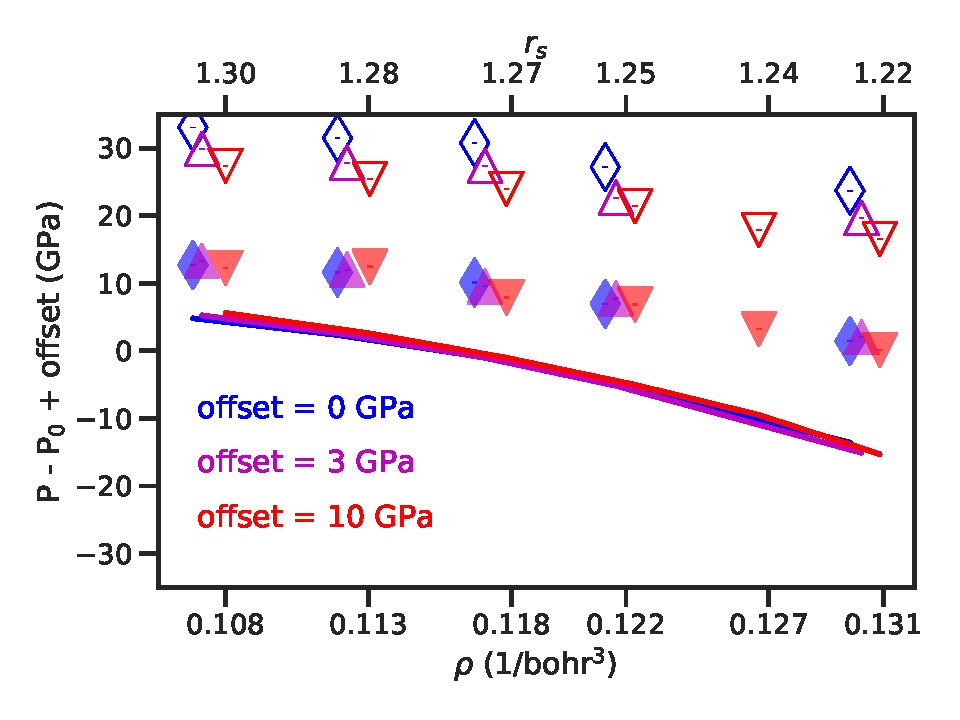
\includegraphics[width=\linewidth]{h117_evp-dynamic-fsc1-rel1-rm121_p-rs}\\
(d) dynamic-lattice relative to $P_0$
\end{minipage}
\caption{Pressure-density relation. The solid lines are clamped-ion vdW-DF pressures, whereas the symbols are QMC pressures. (a) (c) show static-lattice results, while (b) (d) show dynamic lattice results. Color denotes different candidate structures. The open and filled symbols represent VMC and linearly extrapolated DMC estimator results. They overlap on the absolute scale in (a) but can be seen to differ by 1 to 5 GPa on a relative scale in (b). The reference pressure-density relation $P_0=-dE_0/dv$ is calculated from the reference EOS $E_0(1/v)$. The same clamped-ion reference is used for both static-lattice and dynamic-lattice results.}
\label{fig:hsolid-p-vs-n}
\end{figure}

\subsection{Conclusion}
The ordering of the candidate structures from this dynamic-lattice study show similar features as the previous QMC study using vdW-DF geometries and harmonic ZPE~\cite{McMinis2015}.
The Cmca-12 structure is nearly degenerate with C2/c-24 but slightly less stable at low pressures.
There is a transition from C2/c-24 to Cmca-4 around $500$ GPa.
Then a Cmca structure transitions to the I4$_1$/amd atomic structure at a higher pressure.
However, we predict no stability range for the Cmca-12 structure, whereas in Ref.~\cite{McMinis2015}, C2/c-24 transitions to it at $424(3)$ GPa.
The most significant disagreement lies in the atomic phase.
We see the atomic phase becomes more stable relative to C2/c-24 around $610$ GPa, whereas Ref.~\cite{McMinis2015} shows this crossing around $450$ GPa.
Our final prediction for the molecular-to-atomic transition pressure is $660$ GPa, which is significantly higher than the previous experimental report~\cite{Silvera2017}.
However, as already mentioned in Sec.~\ref{sec:hsolid-dep}, this prediction is not unreasonable.
The dynamic-lattice DMC method is a conceptually simple way to directly simulate an electron-ion system and offers more ionic observables as well as direct comparisons with the static-lattice system than a single clamped-ion calculation.
A Born-Oppenheimer study using the DMC energy surface is needed to bridge the previous static-lattice and harmonic ZPE study with the current dynamic-lattice nonadiabatic calculation.
A detailed comparison among the three variants will hopefully resolve some of the disagreements we currently have.

%\subsection{Time Step and Population Control Biases}